\documentclass[11pt,a4paper,english,oneside]{book}

%----------------------------------------------------------------------------------------
% THESIS SETTINGS - ADAPT
%----------------------------------------------------------------------------------------
% Depending on your program, (un)comment the following lines

% Are you in the Quant finance program?
\newif\ifQF % default behaviour is false, so NOT in QF - always leave uncommented!
% \QFtrue % Uncomment if you are in the QF program, if not leave it out


\newcommand{\thesis}{Currency Analysis}



% ==========================================================================================
% PREAMBLE
% ==========================================================================================
%----------------------------------------------------------------------------------------
% GENERAL  - PACKAGES
%----------------------------------------------------------------------------------------
% GENERAL
\usepackage{etex} %Because of many packages --> Extended TeX.
\usepackage[utf8]{inputenc} %Due to vowels.
% \usepackage[british]{babel} %Define the language style.

%Load some mathematical packages.
\usepackage{amsmath}
\usepackage{amsfonts}
\usepackage{amsmath}
\usepackage{amssymb}
\usepackage{mathtools}
\usepackage{breqn} % breaking of equations (be careful with using ENDFLOAT  with this)

%  LAYOUT/PAGE/TEXT FORMATTING
\usepackage[left=1in, right=1in]{geometry} %Helps to structure the paper layout.
\usepackage{setspace} %Use double spacing.

\usepackage[Lenny]{../../styles/fncychap} %Design of the thesis. = Fancy chapter

\usepackage{fancyhdr} %To customize the headers and footers.
\usepackage[hang,bottom,stable,multiple]{footmisc} %Style of footnotes.
\usepackage{dsfont} %Nice style for the indicator function.

\usepackage[svgnames]{xcolor} % Enabling mixing colors and color's call by 'svgnames'
% define new colors (not limited to text obviously)
\definecolor{MyColor1}{rgb}{0.2,0.4,0.6} % mix personal color


% FLOATS
\usepackage{booktabs} %In case you need \cmidrule or \addlinespace in tables.
\usepackage{array} %To create tables and matrices.
\usepackage{hhline}
\usepackage{rotating} %To rotate a table/figure. e.g. \sidewaystable
\usepackage{tabularx} %An extended version of tabular.
\usepackage{float} %Allows for the 'H' option

\usepackage{graphicx} %For the graphics


\usepackage[margin=10pt, font=small, labelfont=bf, labelsep=endash]{caption} %Customize the captions.


% OTHER ENVIRONMENTS


\usepackage{textcomp}

\usepackage{amsthm} %For theorems, definitions etc.
\usepackage{thmtools} %For theorems, definitions etc.

\usepackage{appendix} %For the \appendixpage command.
\usepackage{etoolbox} %To remove the page number on \appendixpage.
\makeatletter %Remove page number on \appendixpage.
\patchcmd{\@chap@pppage}{\thispagestyle{plain}}{\thispagestyle{empty}}{}{}
\makeatother


\usepackage{../../styles/mcode} %To implement Matlab code.
\usepackage{listings} % For including code in your pdf

% VARIA  - does not mean useless
\usepackage{epstopdf} %For inserting .eps files into the document.
\usepackage{lipsum} %For the \lipsum command to generate a text.
\usepackage{datetime} %For the specification of the date.
\usepackage{chngcntr} %To use counterwithout.
\usepackage{xparse} %Load for \NewDocumentCommand command.
\usepackage{arydshln} %Due to the capability to draw horizontal/vertical dash-lines.

%  REFERENCING
% % BIBLIOGRAPHY - BIBTEX
% \usepackage[sort,round]{natbib} %For the bibliography.
% \bibliographystyle{abbrvnat} %Reference style.

% BIBLIOGRAPHY - BIBLATEX
\usepackage[
backend=biber,
style=apa,
bibstyle=authoryear,
citestyle=authoryear,
maxcitenames=2,
maxbibnames=99
]{biblatex}

\setlength\bibitemsep{1\itemsep} % spacing between entries in references
\addbibresource{reference.bib} % .bib file


\usepackage{hyperref} %Must be loaded at the end.
\hypersetup{ %Setup of the reference links.
     colorlinks=false,
     linkcolor=blue,
     citecolor=blue,
     filecolor=magenta,
     urlcolor=blue
}

\usepackage[nameinlink,capitalize]{cleveref} %For the command \cref, load after hyperref.

%----------------------------------------------------------------------------------------
% GENERAL  - SETUP
%----------------------------------------------------------------------------------------
%Define some reasonable margins.
\setlength{\textwidth}{6.6in}
\setlength{\textheight}{8.8in}
\setlength{\topmargin}{-0.1in}
\setlength{\oddsidemargin}{0in}
\setlength{\parskip}{1mm}

\setlength{\parindent}{0cm} %Uncomment this if you don't want to have indents.

%Read just the numbering.
\counterwithout{footnote}{chapter}
\numberwithin{equation}{chapter}

\allowdisplaybreaks[1] %Page breaks of equations are allowed, but avoided if possible. 2-4 more relaxed.

%----------------------------------------------------------------------------------------
% CUSTOM COMMANDS/ENVIRONMENTS
%----------------------------------------------------------------------------------------
%New command for the differential d to have an ordinary d.
\makeatletter
  \newcommand{\ud}{\mathrm{d}}
\makeatother

%Declare Definitions, Theorems etc.(ENVIRONMENTS)
\declaretheorem[style=definition,qed=\(\blacktriangleleft\), numberwithin=chapter]{remark} %additional options; numberwithin=,..., see 'Thmtools' Users’ Guide
\declaretheorem[style=definition,qed=\(\triangle\),numberwithin=chapter]{definition}
\newtheorem{ass}{Assumption}[chapter]
\newtheorem{prop}{Proposition}[chapter]
\newtheorem{lemma}{Lemma}[chapter]
\declaretheorem[style=definition,qed=\(\perp\),numberwithin=chapter]{example}
\newtheorem{theorem}{Theorem}[chapter]
\newtheorem{coroll}{Corollary}[chapter]

%----------------------------------------------------------------------------------------
% TITLE PAGE -  Creates titlepage command
%----------------------------------------------------------------------------------------
%New command for the UZH logo. Used within big \titleGP
\newcommand*{\uzhlogo}{
\includegraphics{../../images/uzh_logo_e_pos.png}}


\newcommand*{\titleGP}{\begingroup %Create the command for including the title page in the document.

\centering %Center all text.

% Include University logo
\vspace*{\baselineskip} %White space at the top of the page.
\ifQF
\uzhlogo\hspace{120pt}\ethlogo\\[2\baselineskip] %University Logo.
\else
\uzhlogo\\[2\baselineskip] %University Logo.
\fi

% Create title 'box'
\rule{\textwidth}{1.6pt}\vspace*{-\baselineskip}\vspace*{2pt} %Thick horizontal line.
\rule{\textwidth}{0.4pt}\\[\baselineskip] %Thin horizontal line.

% TITLE
{\LARGE Which of the G10 currencies is the
riskiest to hold for a Swiss resident?}\\[0.2\baselineskip] %Title.

\rule{\textwidth}{0.4pt}\vspace*{-\baselineskip}\vspace{3.2pt} %Thin horizontal line.
\rule{\textwidth}{1.6pt}\\[2\baselineskip] %Thick horizontal line.
\scshape %Small caps.

% Thesis
\thesis's Thesis\\[2\baselineskip]


\vspace*{2\baselineskip}

% AUTHOR BLOCK - ADAPT
Authors\\
{\Large Yudi  \\ Tane  \\ Migjen   \\ [5pt]
}

\vfill

{\scshape Date of Submission: December 11, 2024} \\[0.3\baselineskip]

\endgroup} % This is the end of the command


%----------------------------------------------------------------------------------------
% HEADER/FOOTER
%----------------------------------------------------------------------------------------
% Special header and footer style for the Executive summary and Task Assignment section.
\fancypagestyle{firststyle}{%
  \fancyhf{}%
  \renewcommand{\headrulewidth}{0pt}
  \fancyfoot[C]{\thepage}
}

%Customize headers and footers. - ADAPT
\pagestyle{fancy}
\fancyhead[R]{\thepage}
\fancyhead[L]{\rightmark}
\fancyfoot[C]{}
\fancyfoot[R]{Currency Analysis} % RUNNING TITLE
\setlength{\headheight}{13.6pt}

%----------------------------------------------------------------------------------------
% SIGNATURE setup
%----------------------------------------------------------------------------------------
%Define the signature line with dots. (create \dotbox command)
\NewDocumentCommand\dotbox{o O{.5\linewidth} m O{3ex} O{\linewidth}}
{
  \begin{minipage}{7cm}
    \makebox[7cm][l]{\,.\dotfill}
    \\
    \makebox[7cm][l]{\,#3}
  \end{minipage}
}
 % CHECK OUT the preamble.tex file and adapt the necessary parts (use CTRL+f and look for "ADAPT"))

\begin{document}

%----------------------------------------------------------------------------------------
% Title
%----------------------------------------------------------------------------------------
\thispagestyle{empty}
\titleGP\

\newpage

\doublespacing\
\setcounter{page}{1}
\pagenumbering{Roman}

{\LARGE \textbf{Abstract}}

This study analyzes exchange rate risks for Swiss investors, focusing on G10 currencies using four risk metrics: depreciation, volatility, maximum drawdown, and Value at Risk (VaR). The Japanese Yen emerged as the riskiest currency due to steep depreciation (-162.21\%) and pronounced volatility. Similarly, the Norwegian Krone demonstrated high vulnerability to global shocks, while the Euro exhibited the lowest risks, reflecting its stability and strong economic integration. The research emphasizes the importance of multidimensional risk evaluation for informed decision-making. Future studies could incorporate broader datasets, geopolitical risks, and machine learning to refine forecasting and enhance risk assessment accuracy.


\pagenumbering{arabic}

\tableofcontents
\listoffigures



\pagenumbering{arabic}

\chapter{Introduction}

Exchange rate risk is vital for Swiss investors, particularly for those possessing assets or debts in foreign currencies. Fluctuations in currency exchange rates can lead to considerable alterations in the worth of investments, savings, or international transactions. Comprehending these risks is crucial for both individuals and organizations, especially for residents of Switzerland who frequently engage with currencies from the G10 alliance. This collection includes some of the most frequently exchanged and economically important currencies worldwide. The compact nature and transparent framework of the Swiss economy, which significantly relies on international trade and financial markets, intensifies the uncertainties linked to foreign currencies \parencite{frohm2024strengthening}. Therefore, evaluating and handling exchange rate risks is essential for making financial choices.

Among the key measures to evaluate currency risk is depreciation, which quantifies the long-term loss in value of a foreign currency relative to the Swiss Franc. This metric is particularly relevant for long-term investors, as it captures the overall financial impact of adverse currency movements over extended periods. Currencies with high cumulative depreciation often indicate structural economic weaknesses or unfavorable exchange rate policies, making them less attractive to Swiss investors. Depreciation provides a cumulative perspective on risk, complementing more dynamic measures like volatility.

Volatility, another critical risk metric, measures the degree of fluctuations in a currency’s value over time. Elevated volatility reflects higher uncertainty and indicates a greater likelihood of significant and unpredictable price changes. For example, a currency with high volatility is more likely to experience sharp movements due to economic or political events, leading to potential gains or losses for investors. Volatility is often considered a foundational measure of financial asset stability and forms the basis for more complex risk evaluations \parencite{poon2003forecasting}.

Maximum Drawdown offers a different perspective by identifying the greatest historical decline in a currency's value, from its peak to its trough, over a specified timeframe. Unlike statistical measures, this metric directly highlights real-life risks by showing the worst-case scenario an investor could have experienced when holding a currency. For instance, a currency that has suffered significant drawdowns in the past may signal vulnerability to economic disruptions or market volatility, making it less appealing to risk-averse investors \parencite{geboers2023peak}.

Finally, Value at Risk (VaR) serves as a statistical tool to estimate potential losses under typical market conditions. At a 95\% confidence level, VaR indicates the maximum expected loss over a defined timeframe, with a 5\% probability of exceeding this threshold. Unlike volatility, which measures the extent of price fluctuations, VaR focuses on the likelihood and magnitude of downside risk, making it a practical tool for risk-averse investors and financial institutions seeking to manage potential losses \parencite{poon2003forecasting}.

Together, these four metrics—depreciation, volatility, maximum drawdown, and Value at Risk—provide a comprehensive framework for evaluating currency risks. Depreciation highlights long-term trends, while the other measures capture short-term variability, historical performance, and potential losses under normal conditions. For Swiss investors, who frequently engage with foreign currencies for investments, trade, or travel, this multidimensional approach offers essential insights to navigate exchange rate uncertainties effectively. By applying these metrics to the G10 currencies, including the US Dollar, Euro, and British Pound, this study provides critical risk assessments that inform broader financial planning and portfolio management.

\chapter{Methodology}
This section describes the approach used to evaluate the risk associated with G10 currencies for Swiss residents. The dataset contains daily exchange rates for G10 currencies relative to the Swiss Franc (CHF) from 2000 to 2024, obtained from Investing.com. These currencies represent a selection of the most actively exchanged and stable economies globally, including the Australian Dollar (AUD), Canadian Dollar (CAD), Euro (EUR), British Pound (GBP), Japanese Yen (JPY), Norwegian Krone (NOK), New Zealand Dollar (NZD), Swedish Krona (SEK), and United States Dollar (USD). The extensive span of nearly 25 years ensures that the analysis covers a broad range of economic cycles, market upheavals, and geopolitical influences.

To evaluate the relative risk associated with these currencies, four important risk metrics were computed: depreciation, volatility, Value at Risk (VaR), and maximum drawdown. These measurements offer an extensive perspective on the risk profiles of the currencies, with each emphasizing a distinct facet of financial risk.

Depreciation, the newly incorporated metric, assesses the cumulative long-term loss in the value of a foreign currency relative to the Swiss Franc. This measure highlights structural vulnerabilities and offers insights into the overall financial consequences of adverse currency movements over time. Depreciation is determined by the percentage variation between the beginning and ending values of the exchange rate throughout the observation period. It acts as a vital addition to other metrics, especially for long-term risk evaluation, since it identifies patterns that might not be readily visible in volatility or drawdown evaluations.

Volatility quantifies the degree of price changes, providing information about the extent of uncertainty or variability in currency shifts. In particular, the annualized standard deviation of the log-returns was computed. Log-returns, calculated as the natural logarithm of consecutive price ratios, are widely used in financial analysis due to their ability to model compounding effects and provide a more accurate depiction of percentage changes over time \parencite{scrucca2024entropy}. By annualizing the standard deviation, we create a standardized metric that allows for comparison across various currencies, irrespective of their trading frequency. Elevated volatility indicates heightened uncertainty and, therefore, an augmented potential risk for investors \parencite{kongsilp2017volatility}.

The second metric, Value at Risk (VaR), measures the possible loss an investor might encounter at a certain probability within a defined time frame. In this research, we utilized the historical method, a non-parametric technique that does not presuppose a particular distribution of returns. The VaR at a 95\% confidence level was determined, indicating that 5\% of the recorded daily returns fall beneath the calculated VaR limit. This measurement is especially beneficial for managing risks, as it establishes a distinct limit for possible losses in regular market circumstances \parencite{manganelli2001value}. In contrast to volatility that assesses variability, VaR concentrates on downside risk, which makes it especially pertinent for risk-averse investors \parencite{artzner1999coherent}.

The third metric, maximum drawdown, measures the greatest drop from a peak to a trough in currency values during the designated time frame. It is an essential metric for evaluating the worst-case situation of possessing a currency, indicating the most significant and lasting drop an investor might have experienced. The maximum drawdown was calculated by initially pinpointing the rolling peak values of the exchange rate and subsequently figuring out the largest percentage decline from any peak to a following trough. This metric underscores a currency's strength in the face of severe market situations, including economic downturns or geopolitical turmoil \parencite{stan2014computation}.

Through the combination of these four metrics, we gained a multidimensional understanding of the risks associated with each currency. Depreciation added a crucial long-term perspective, highlighting the cumulative effects of adverse currency movements, particularly for currencies like the Japanese Yen and British Pound, which demonstrated significant depreciation over the analyzed periods. This comprehensive approach enables us to compare their behavior under varying market conditions, ultimately addressing the research question of identifying the riskiest G10 currency for Swiss residents.
\chapter{Analysis}
\section{Pre-Global Financial Crisis (2000–2007)}
In the times preceding the Global Financial Crisis, the G10 currencies displayed varying levels of risk when evaluated using the indicators of depreciation, volatility, Value at Risk (VaR), and maximum drawdown.

\begin{figure}[h!]
    \centering
    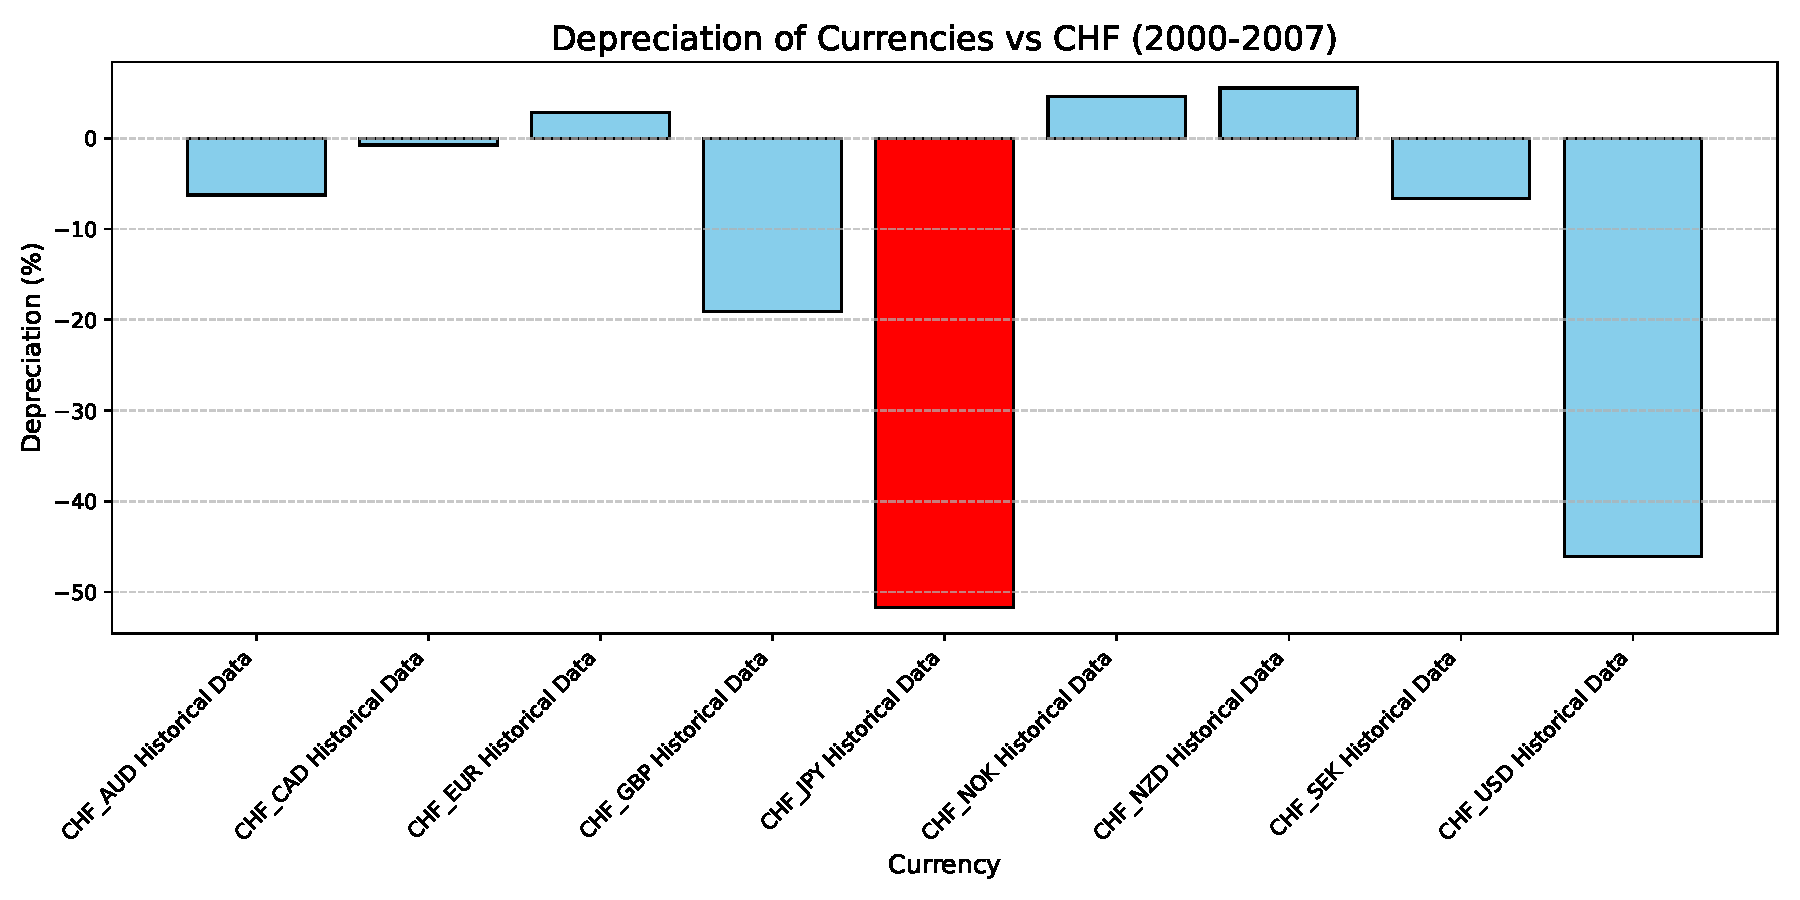
\includegraphics[width=0.75\textwidth]{../../images/depreciation_2000_2007.pdf}
    \caption{Depreciation of Currencies vs CHF (2000--2007).}
    \label{fig:depreciation_2000_2007}
\end{figure}

Depreciation results reveal that the Japanese Yen experienced substantial depreciation relative to the Swiss Franc during this period, highlighting the relative strengthening of the Swiss Franc. Similarly, the US Dollar faced significant depreciation, reflecting vulnerabilities tied to broader economic conditions. In contrast, the Euro demonstrated an appreciation, underscoring its stability and the initial confidence associated with its introduction as a global currency \parencite{EuropeanUnion2024}. The Norwegian Krone and the New Zealand Dollar also gained appreciation.

\begin{figure}[h!]
    \centering
    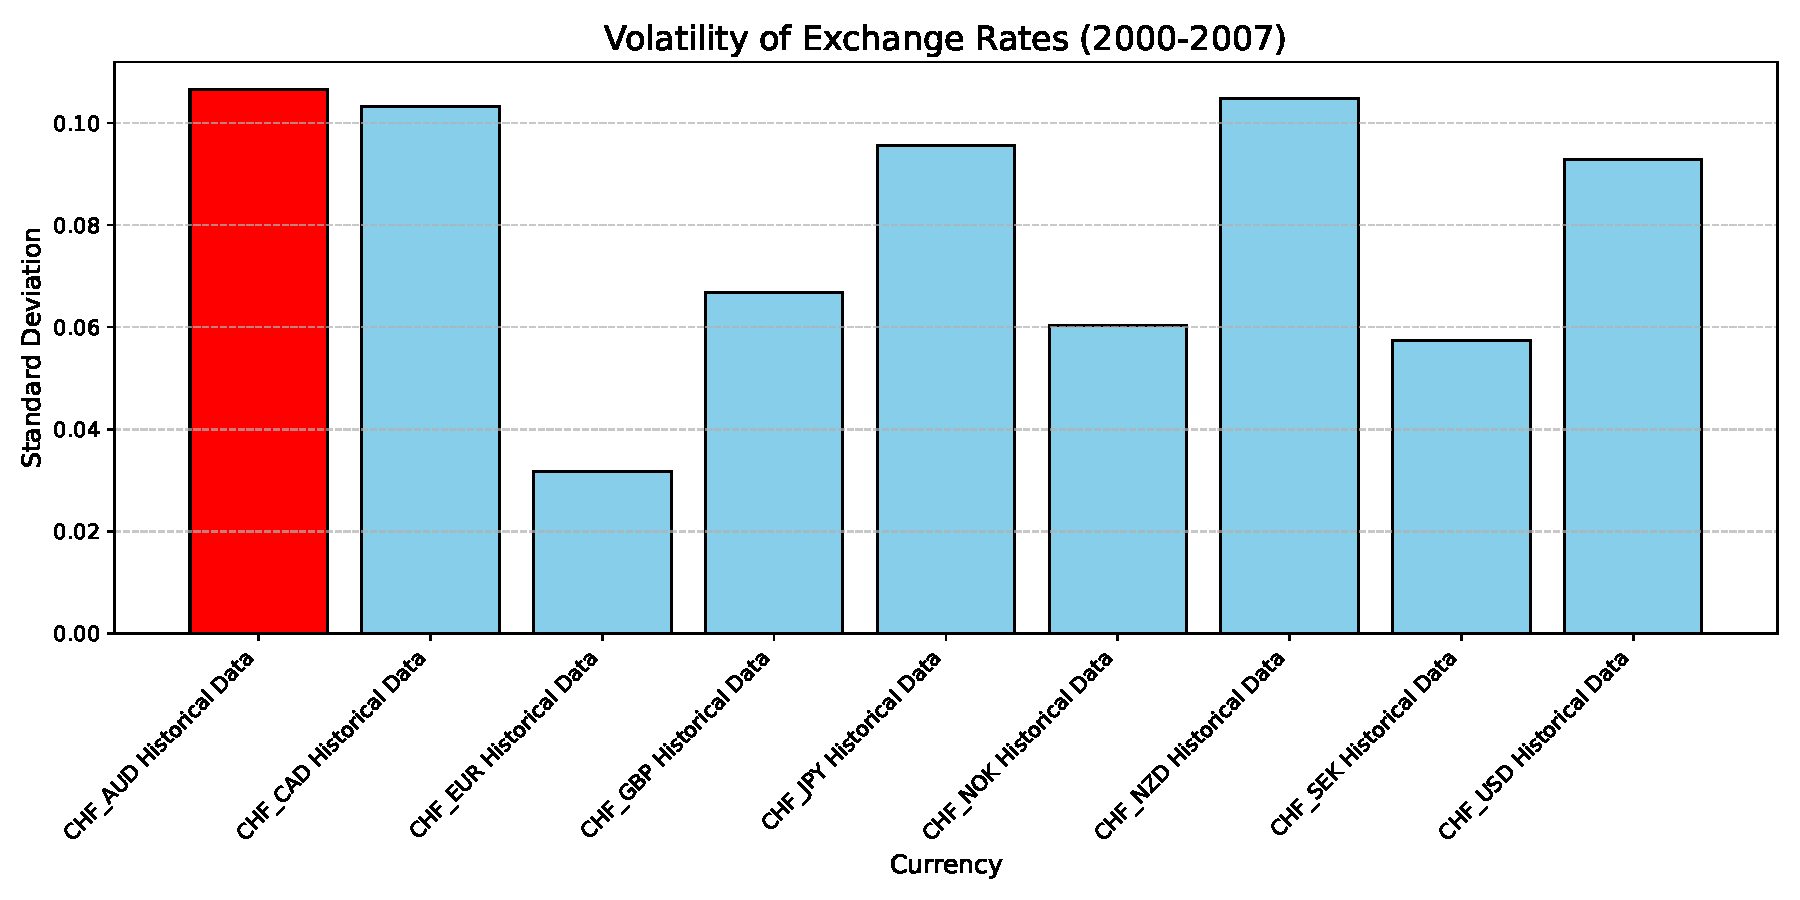
\includegraphics[width=0.75\textwidth]{../../images/volatility_2000_2007.pdf}
    \caption{Volatility of Exchange rates (2000--2007).}
    \label{fig:volatility_2000_2007}
\end{figure}

Volatility indicates that the Australian Dollar displayed the highest standard deviation, making it the most volatile currency in this period. This heightened volatility is often attributed to Australia's reliance on commodity exports and its open economy, which exposed it to external market shocks \parencite{chen2003commodity}. Conversely, the Euro exhibited lower volatility, reinforcing its reputation as a stable currency supported by strong economic frameworks within the eurozone \parencite{juncker2015completing}.

\begin{figure}[h!]
    \centering
    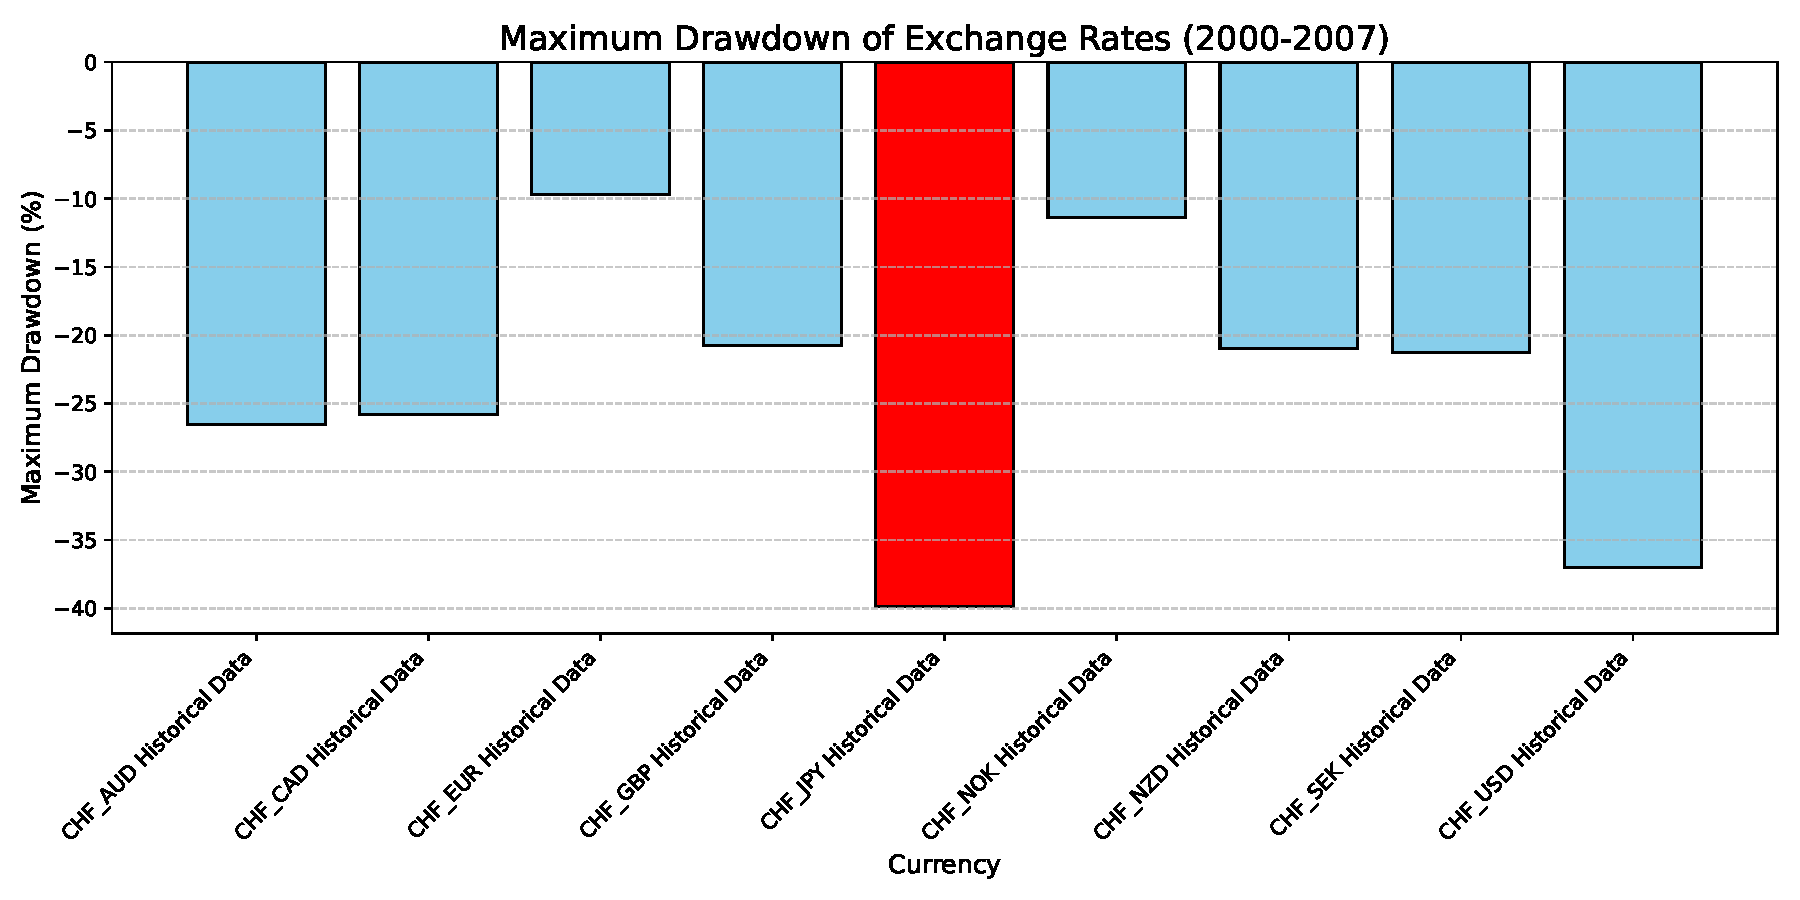
\includegraphics[width=0.75\textwidth]{../../images/maximum_drawdown_2000_2007.pdf}
    \caption{Maximum Drawdown of Exchange rates (2000--2007).}
    \label{fig:maximum_drawdown_2000_2007}
\end{figure}

The maximum drawdown analysis underscores critical differences in historical risks. The Japanese Yen experienced significant drawdowns during this period, challenging its traditional status as a safe-haven currency \parencite{kopyl2016safe}. Similarly, the US Dollar faced substantial drawdowns, reflecting vulnerabilities associated with global monetary shifts. In contrast, the Euro experienced smaller drawdowns, reinforcing its role as a stable currency during this era.

\begin{figure}[h!]
    \centering
    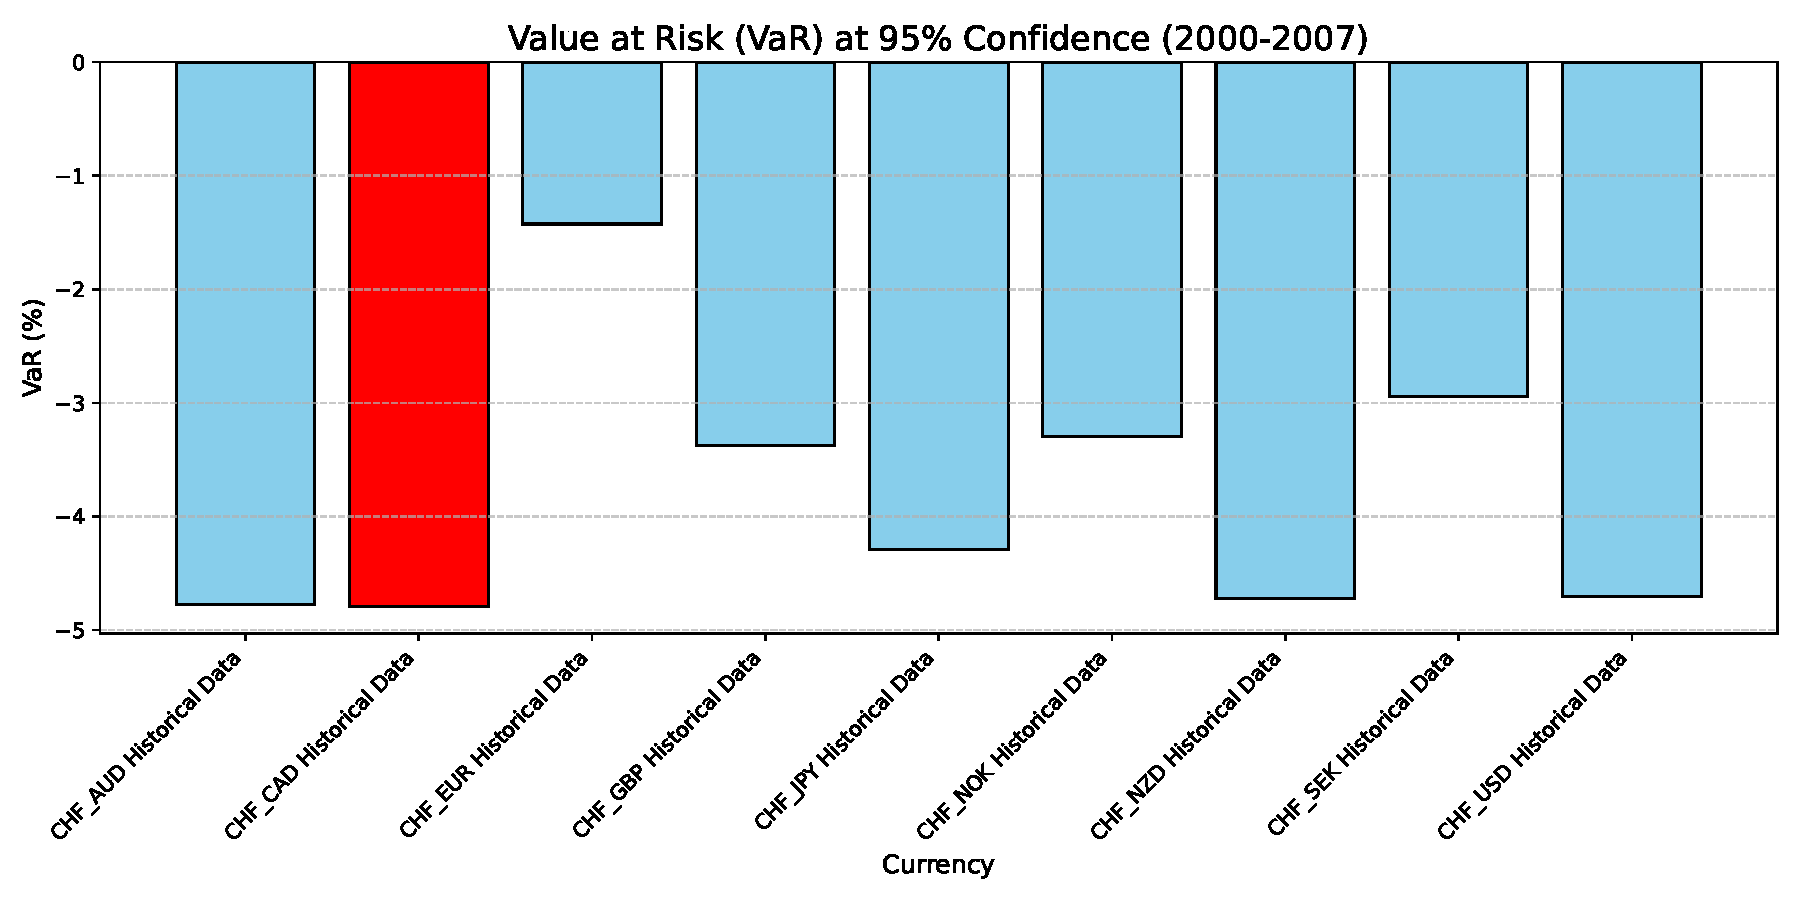
\includegraphics[width=0.75\textwidth]{../../images/var_2000_2007.pdf}
    \caption{Value at Risk of Exchange rates (2000--2007).}
    \label{fig:var_2000_2007}
\end{figure}

Analyzing Value at Risk (VaR) provides additional insights into potential downside risks. The Euro stands out as the least risky currency, demonstrating minimal expected losses under typical market conditions. On the other hand, the Canadian Dollar displayed higher VaR levels, consistent with its sensitivity to global commodity price fluctuations due to Canada's heavy reliance on energy exports \parencite{chen2003commodity}.

By synthesizing these metrics, a nuanced picture of currency risks emerges. The Japanese Yen, despite its safe-haven reputation, exhibited high drawdowns and depreciation, challenging its conventional stability narrative. Similarly, the Australian and US Dollars emerged as riskier options due to their elevated volatility, drawdowns, and less favorable depreciation profiles. In contrast, the Euro showcased consistently lower risks across all metrics, reflecting its growing role as a reserve currency and its association with economic stability.

\section{During the Global Financial Crisis (2007–2009)}
The period of the Global Financial Crisis (2007–2009) represented one of the most tumultuous periods in modern economic history, noted for severe market drops and significant fluctuations in exchange rates. This segment assesses the risk metrics—depreciation, volatility, Value at Risk (VaR), and maximum drawdown—for the G10 currencies throughout this chaotic phase.

\begin{figure}[h!]
    \centering
    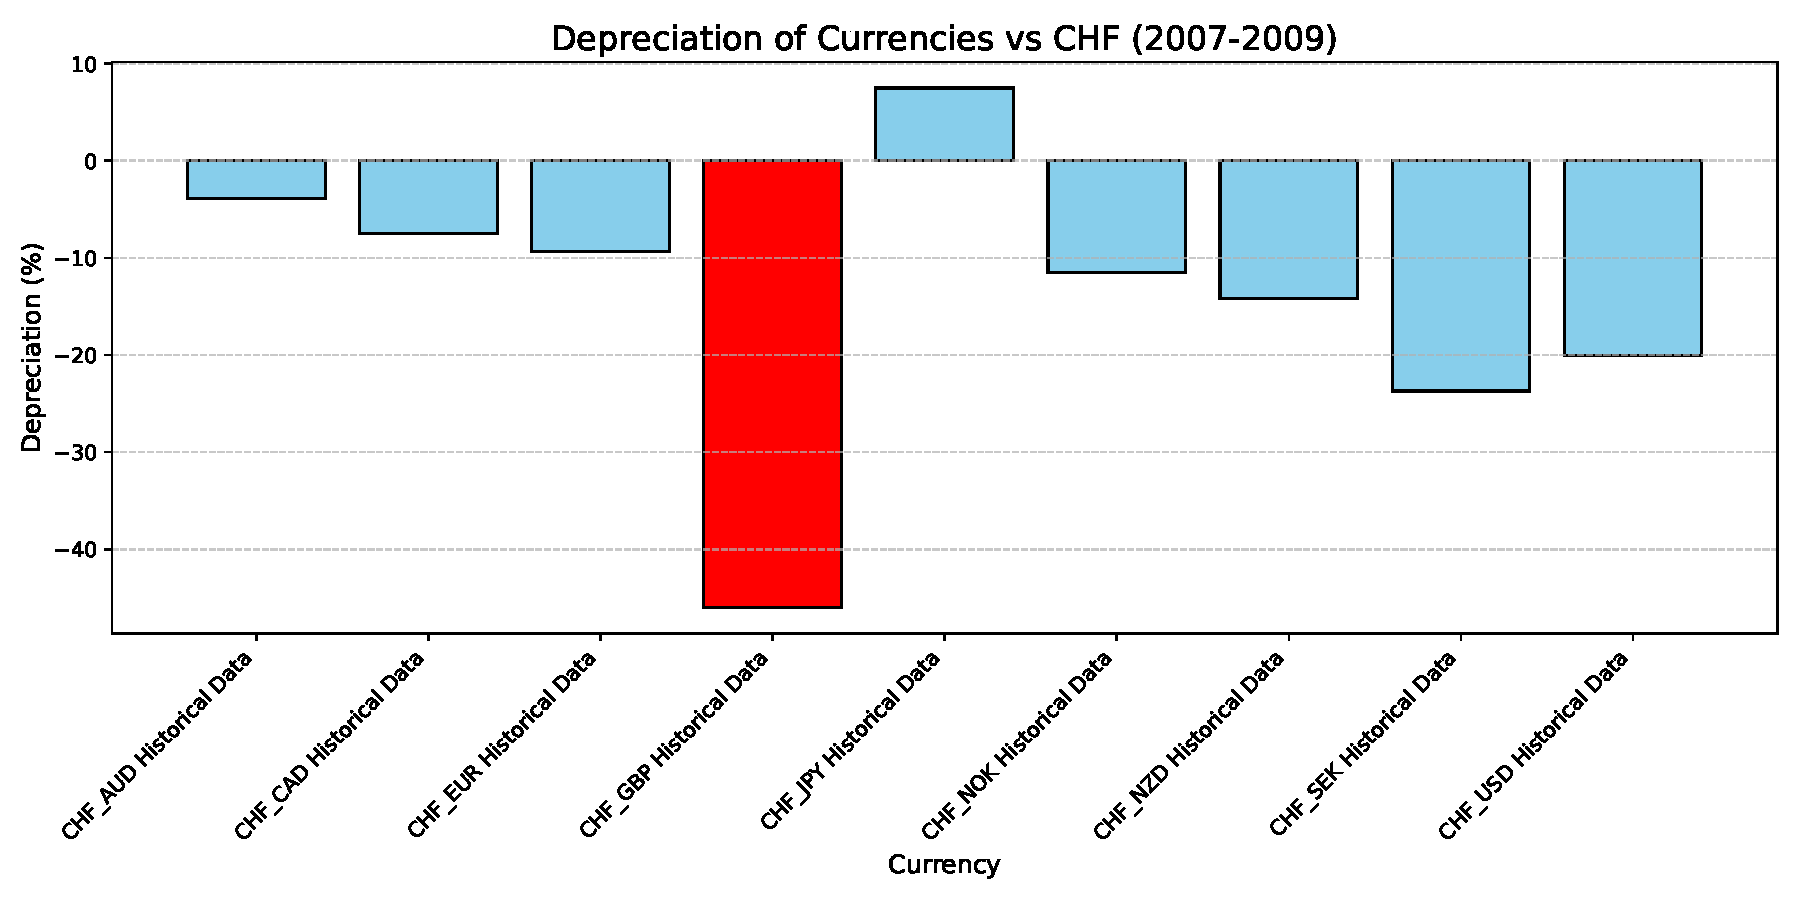
\includegraphics[width=0.75\textwidth]{../../images/depreciation_2007_2009.pdf}
    \caption{Depreciation of Currencies vs CHF (2007--2009).}
    \label{fig:depreciation_2007_2009}
\end{figure}

Depreciation findings indicate that the British Pound experienced the most significant depreciation (-45.99\%) compared to the Swiss Franc. This demonstrates the profound effects of the financial crisis on the economy of the United Kingdom, which was significantly influenced by global financial markets. On the other hand, the Japanese Yen showed an increase of 7.50\%, highlighting its status as a safe-haven currency in times of economic turmoil. The Euro showed notable strength, experiencing a slight decline of -9.32\%, underscoring the relative stability of the eurozone during significant economic upheavals. These results highlight the differing levels of currency stability and the unique effects of the crisis on various economies.

\begin{figure}[h!]
    \centering
    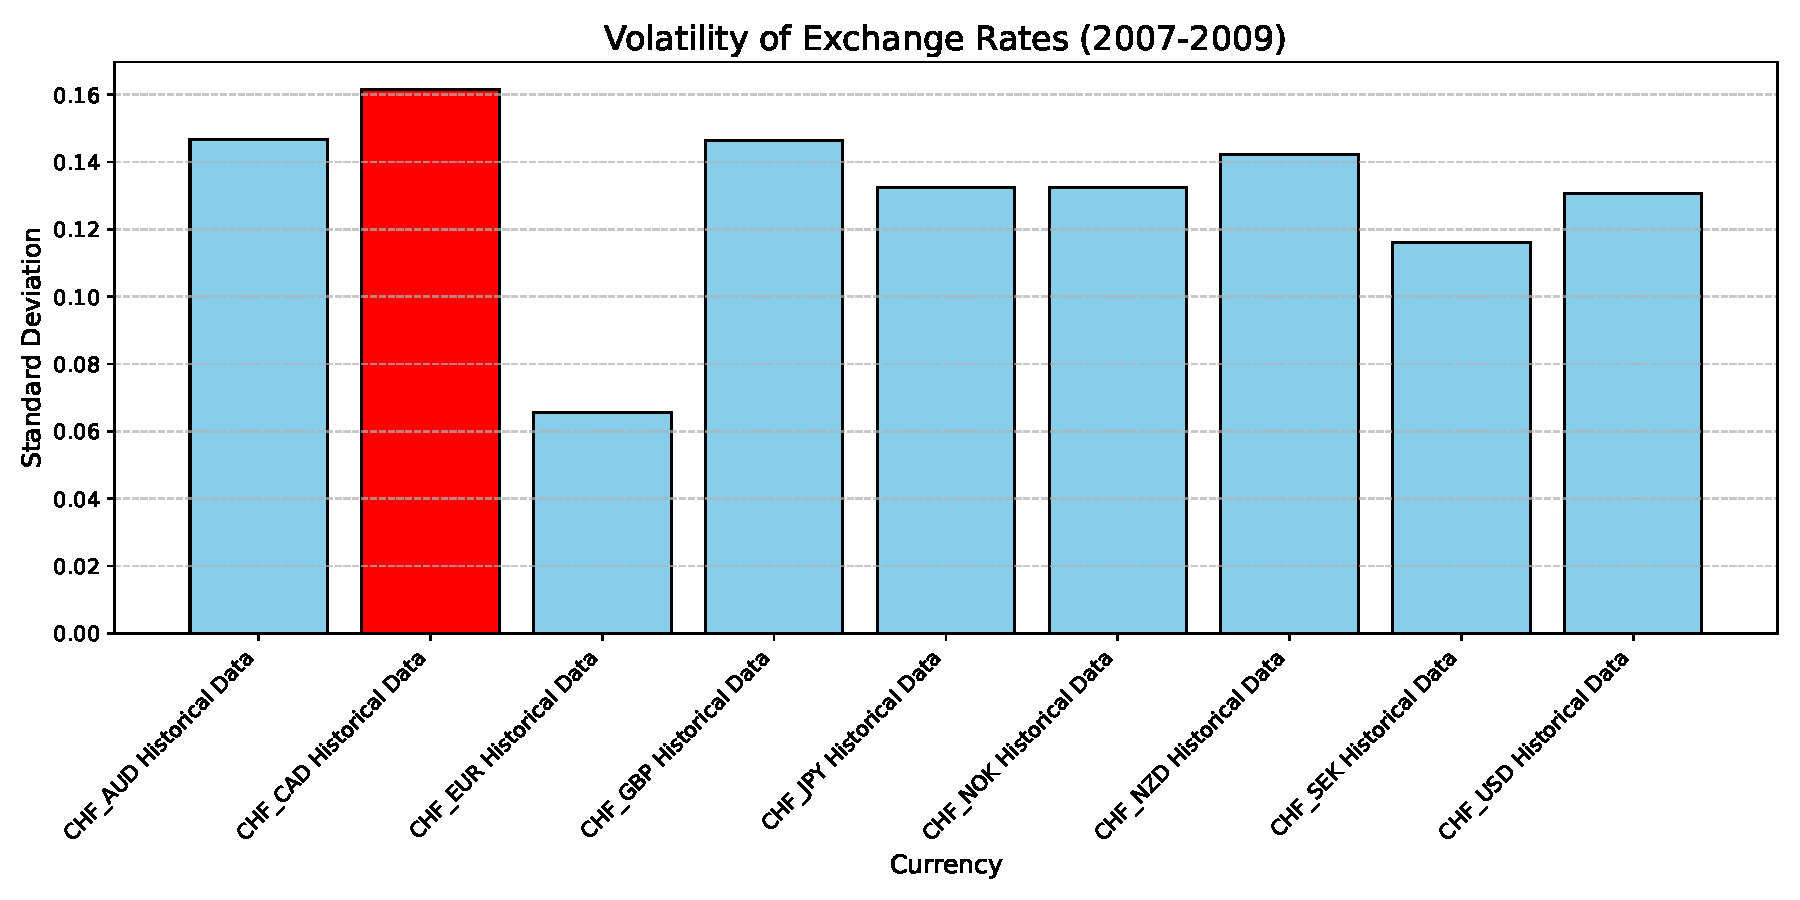
\includegraphics[width=0.75\textwidth]{../../images/volatility_2007_2009.pdf}
    \caption{Volatility of Exchange rates (2007--2009).}
    \label{fig:volatility_2007_2009}
\end{figure}

The volatility chart reveals that the CHF-CAD and CHF-AUD currency exchange rates exhibited the highest levels of variation, displaying standard deviations of 0.1616 and 0.1468, correspondingly. This heightened volatility is due to Canada and Australia being countries that export commodities, having economies closely linked to international trade. Throughout the financial crisis, the oil price shock led to extreme volatility as the price went up to almost 150\$ per barrel in the summer and back to 40\$ in December \parencite{behr20092008}. This may have caused the currency of commodity-exporting countries to vary. In comparison, the CHF-EUR exchange rate displayed the lowest volatility at 0.0655, underscoring the eurozone's relative stability despite difficulties in other international markets. The euro's relative stability mirrors synchronized monetary policies and strong economic fundamentals in the eurozone \parencite{lane2012european}.

\begin{figure}[h!]
    \centering
    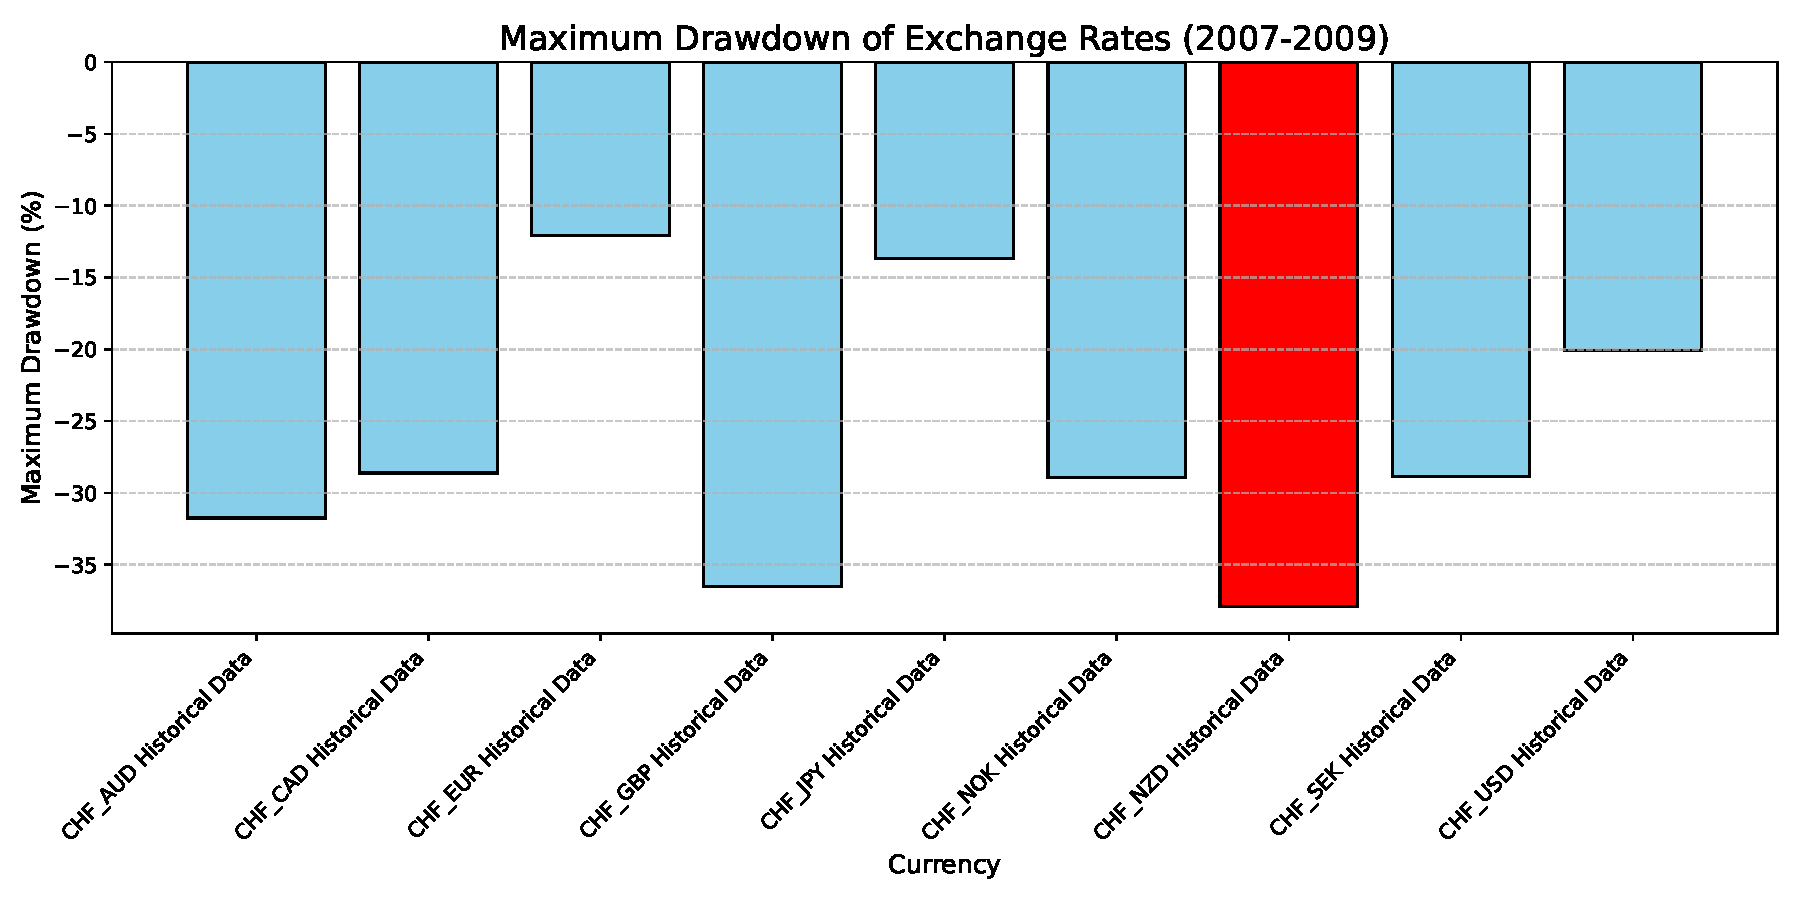
\includegraphics[width=0.75\textwidth]{../../images/maximum_drawdown_2007_2009.pdf}
    \caption{Maximum Drawdown of Exchange rates (2007--2009).}
    \label{fig:maximum_drawdown_2007_2009}
\end{figure}

The maximum drawdown measure provides a deeper perspective into the historical severity of currency declines during the crisis. The CHF-NZD exchange rate experienced the largest drawdown at -37.88\%, reflecting significant investor pessimism and the vulnerability of the New Zealand economy to systemic financial shocks. The GBP followed closely with a drawdown of -36.51\%, underscoring the impact of declining global trade on smaller, export-driven economies. Conversely, the Euro had the smallest maximum drawdown at -12.10%.

\begin{figure}[h!]
    \centering
    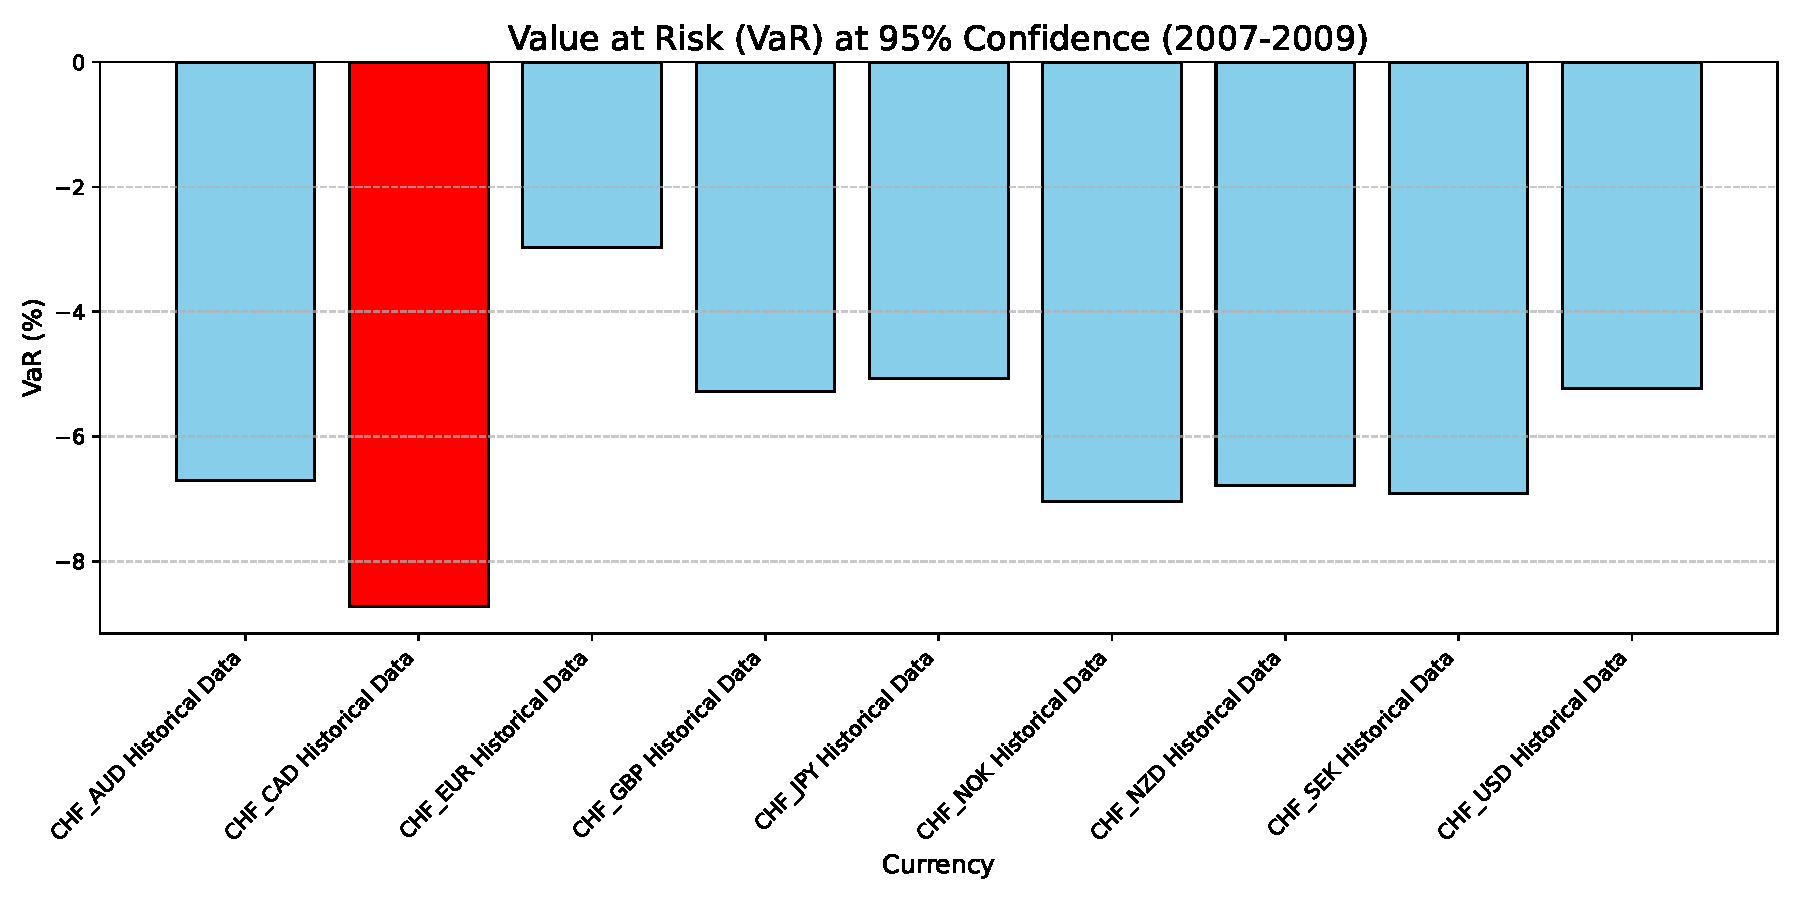
\includegraphics[width=0.75\textwidth]{../../images/var_2007_2009.pdf}
    \caption{Value at Risk of Exchange rates (2007--2009).}
    \label{fig:var_2007_2009}
\end{figure}

The Value at Risk (VaR) assessment supports these findings, indicating that the CHF-CAD demonstrated the highest VaR at -8.72\%, signifying the substantial risks associated with holding this currency during the crisis. This aligns with the economic vulnerabilities Canada faced as an economy strongly tied to the US economy, where the financial crisis originated and had the biggest impact \parencite{claessens2010cross}. Similarly, CHF-AUD exhibited a significant VaR of -6.71\%, reinforcing the heightened risks associated with commodity-linked currencies. In contrast, the CHF-EUR demonstrated the lowest VaR at -2.98\%, showcasing its comparative stability during this period of financial turbulence.

Synthesizing all four metrics provides a comprehensive view of currency risks during the Global Financial Crisis. The British Pound emerged as one of the riskiest currencies, with the highest depreciation and maximum drawdown. In contrast, the Japanese Yen demonstrated exceptional resilience across all metrics, bolstered by its safe-haven status and investor confidence during periods of uncertainty. The Euro, while experiencing moderate depreciation, remained relatively stable, reflecting strong economic fundamentals and coordinated eurozone policies.

In conclusion, the analysis highlights the heightened risks associated with currencies from commodity-exporting countries, such as the Canadian, Australian, and New Zealand Dollars, which were disproportionately affected by the financial crisis due to their dependency on global trade. Conversely, safe-haven currencies like the Japanese Yen and economically integrated currencies like the Euro exhibited greater stability, offering insights into the broader economic and monetary strategies that shaped currency risks during this unprecedented financial turbulence.

\section{Post-Financial Crisis (2009–2024)}
Following the 2008 financial crisis, global financial markets experienced a phase of stabilization, but certain currencies displayed heightened levels of volatility and risk, reflecting regional economic events and global monetary policies. During this period, the metrics of depreciation, volatility, maximum drawdown, and Value at Risk (VaR) reveal significant trends among the G10 currencies.

\begin{figure}[h!]
    \centering
    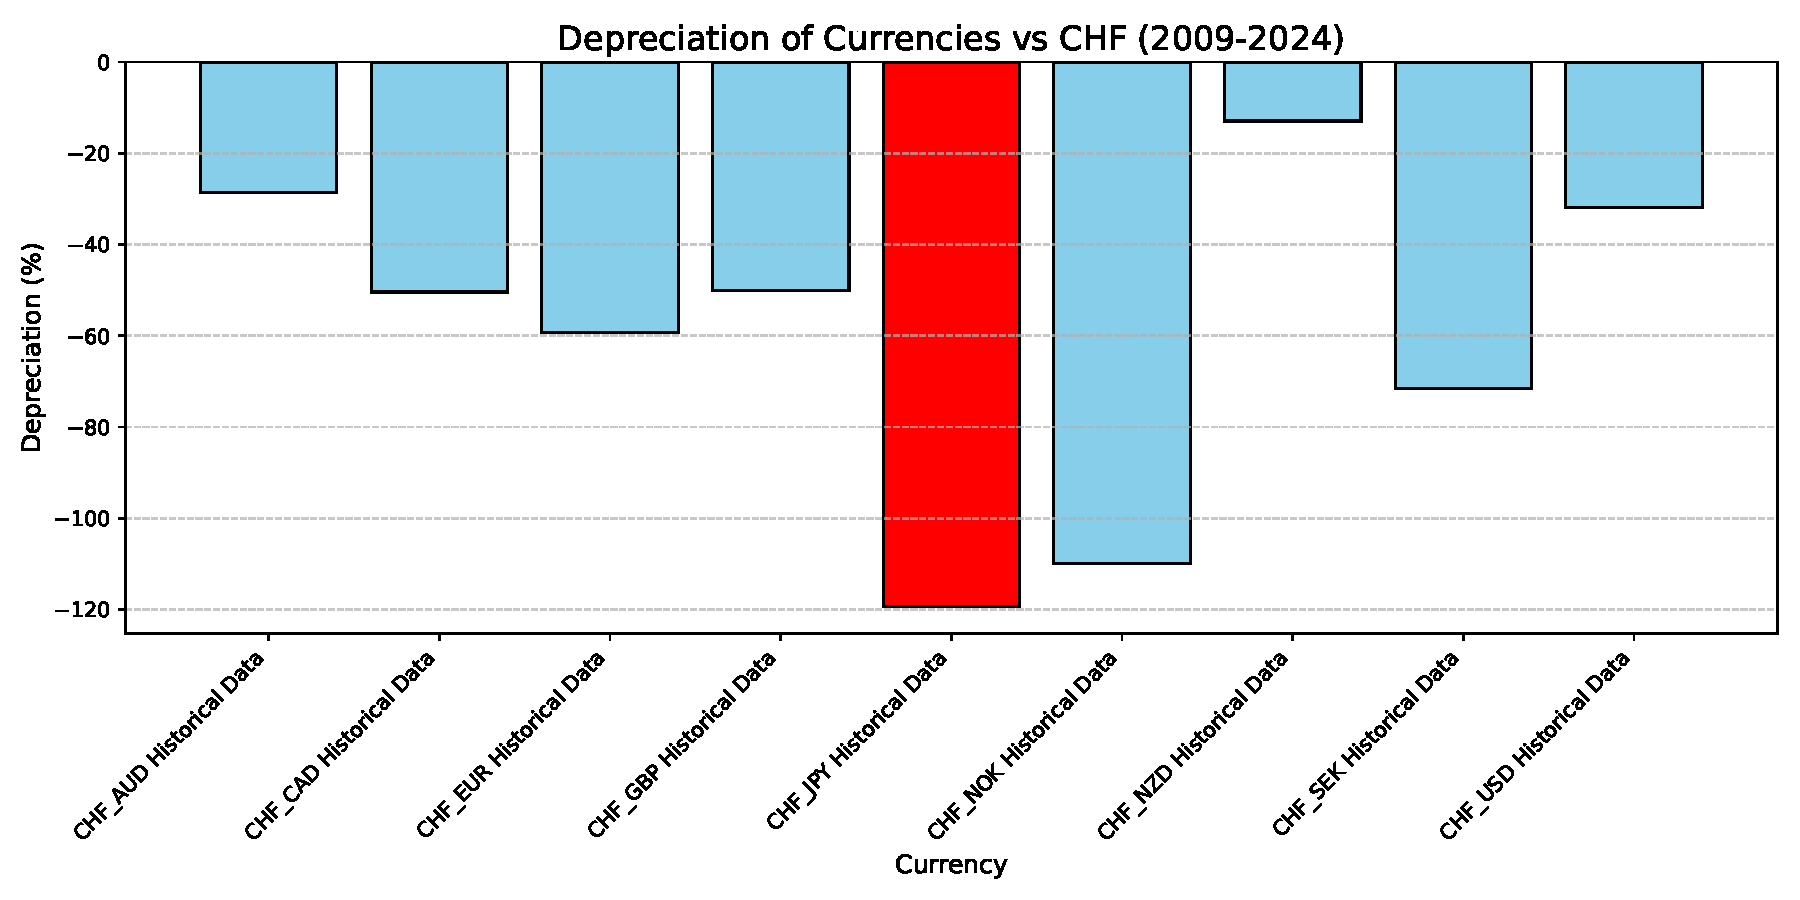
\includegraphics[width=0.75\textwidth]{../../images/depreciation_2009_2024.pdf}
    \caption{Depreciation of Currencies vs CHF (2009--2024).}
    \label{fig:depreciation_2009_2024}
\end{figure}

The depreciation analysis indicates that the Japanese Yen faced the largest depreciation, registering a total decline of -119.28\% in relation to the Swiss Franc. This outcome highlights the ongoing weakness of the JPY compared to the CHF, likely affected by Japan's extraordinarily lenient monetary policies, including negative interest rates and significant quantitative easing by the Bank of Japan (BOJ). These measures, aimed at boosting local demand, also devalued the currency through expanded monetary supply \parencite{shirai2020bank}. In contrast, the New Zealand Dollar showed the least depreciation at -12.94\%, reflecting its relative resilience during this period.

\begin{figure}[h!]
    \centering
    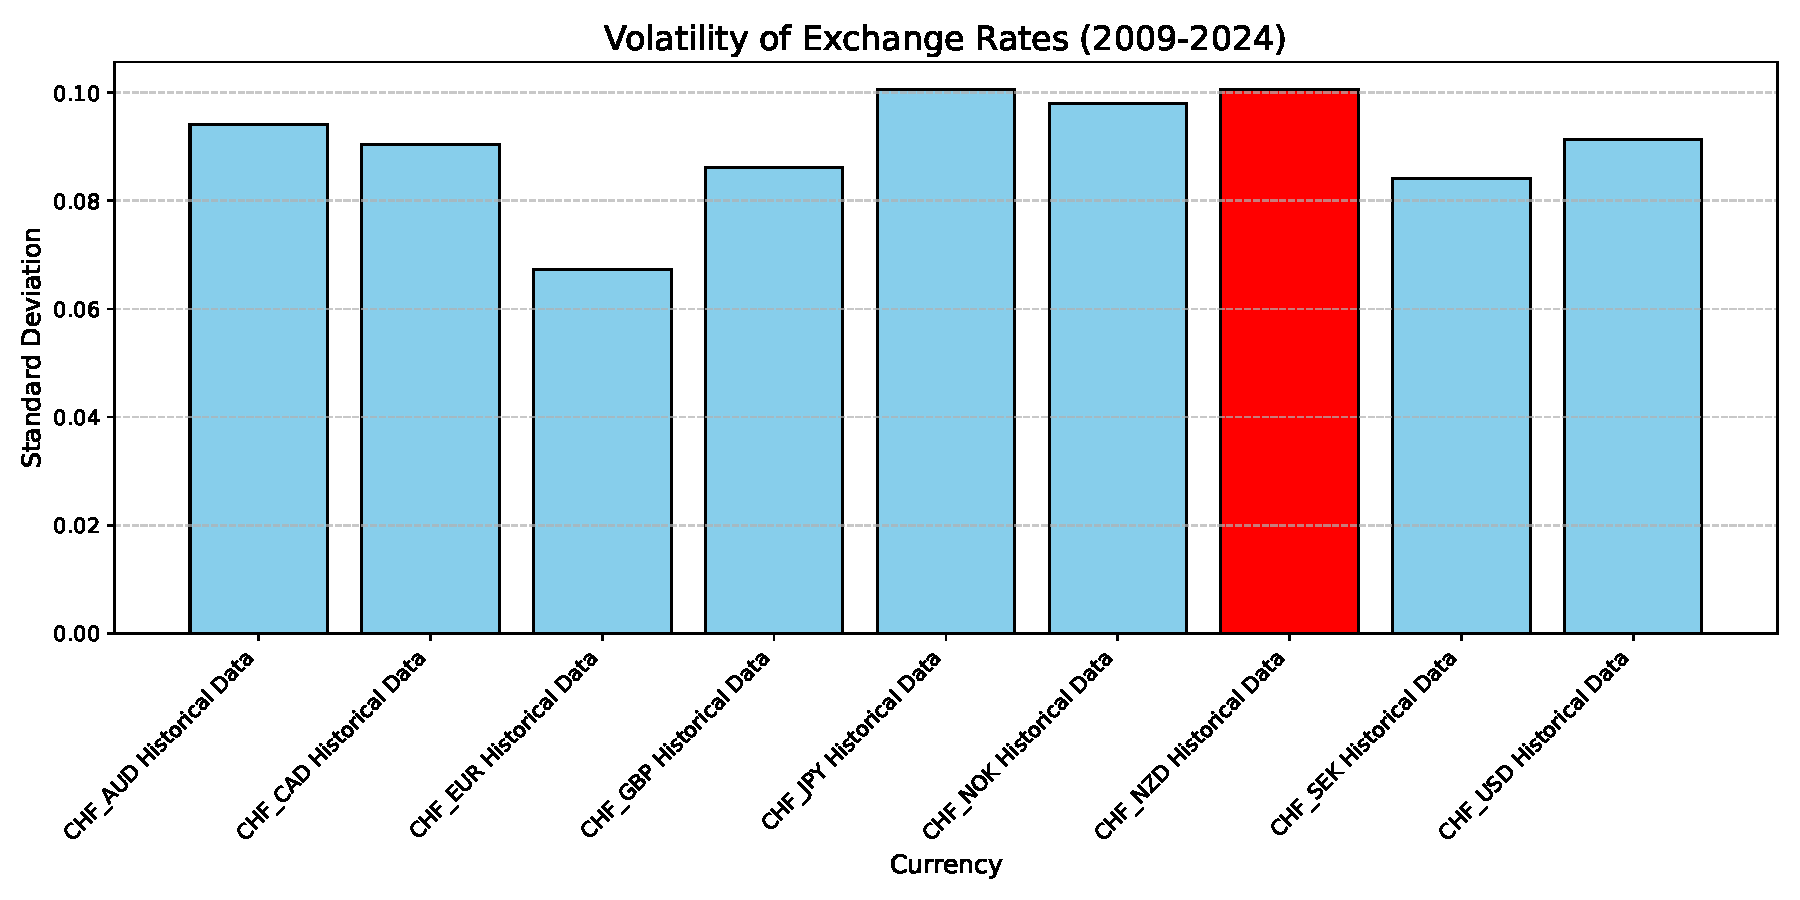
\includegraphics[width=0.75\textwidth]{../../images/volatility_2009_2024.pdf}
    \caption{Volatility of Exchange rates (2009--2024).}
    \label{fig:volatility_2009_2024}
\end{figure}

The volatility examination reveals that the New Zealand Dollar and Japanese Yen had the greatest standard deviation values, around 0.101 and 0.100 respectively. The NZD's considerable volatility underscores its dependence on agricultural exports and susceptibility to changes in global commodity prices. Conversely, the JPY's volatility results from its dual role as a safe-haven currency and its vulnerability to speculative trading during uncertain financial times. The Euro had the lowest volatility during this time frame (0.0674), consistent with the eurozone's monetary stability, as well as Switzerland's steady economic alignment with the eurozone \parencite{claessens2010cross}.

\begin{figure}[h!]
    \centering
    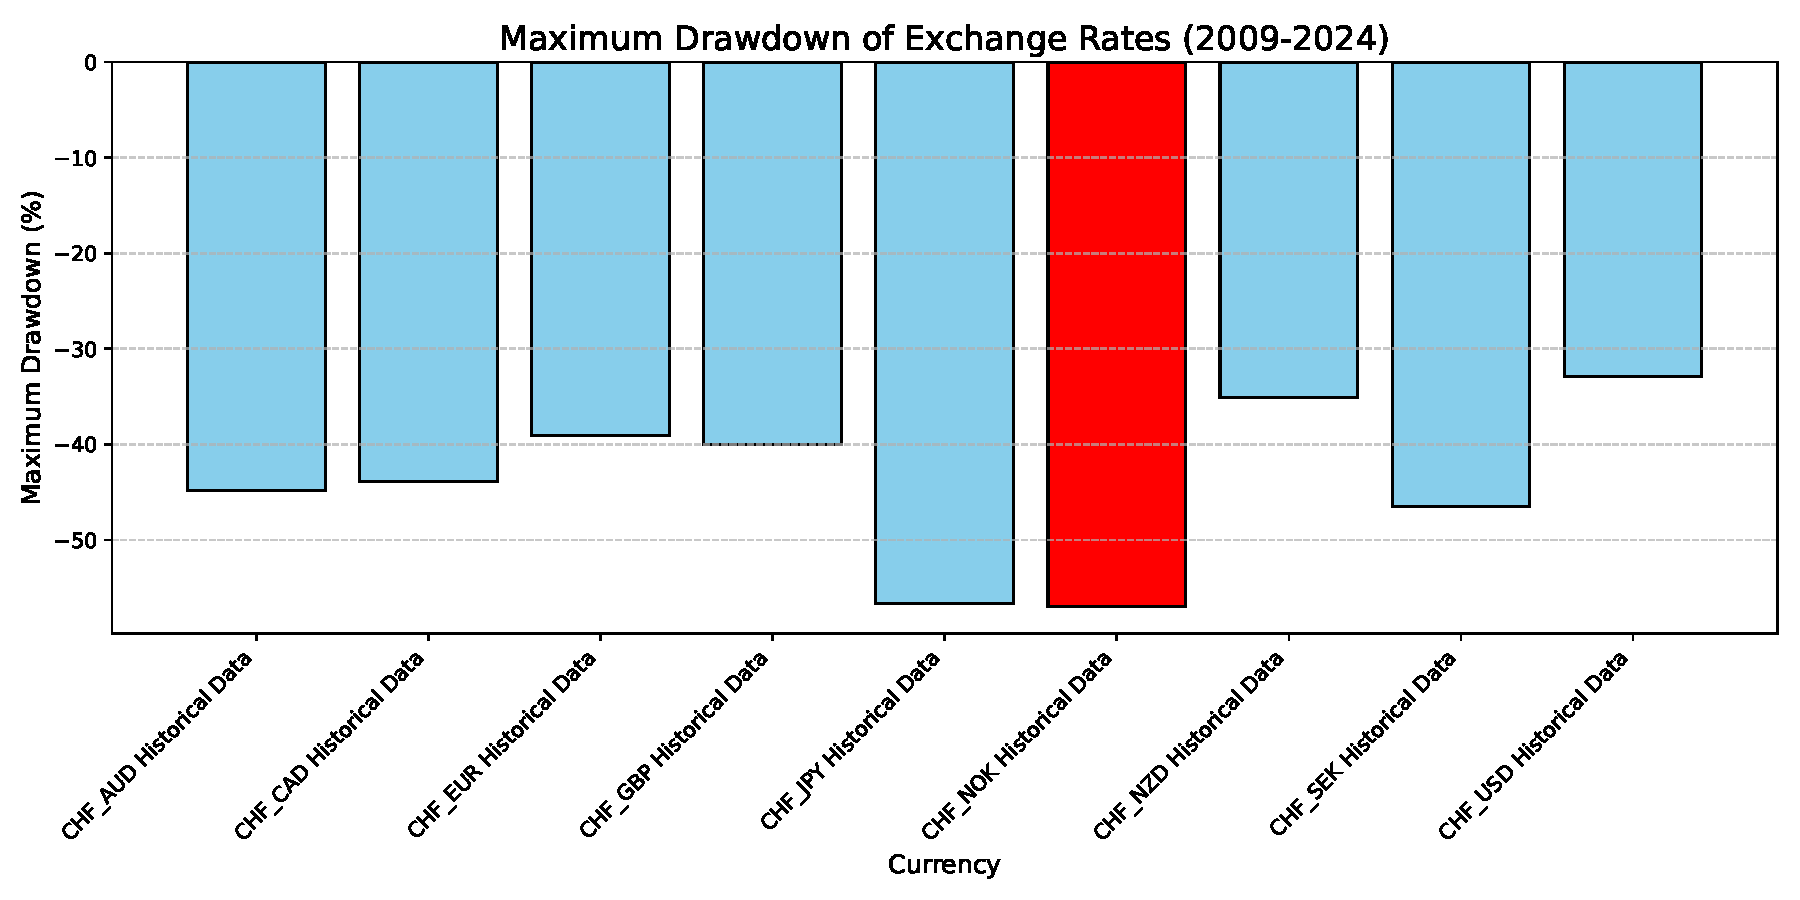
\includegraphics[width=0.75\textwidth]{../../images/maximum_drawdown_2009_2024.pdf}
    \caption{Maximum Drawdown of Exchange rates (2009--2024).}
    \label{fig:maximum_drawdown_2009_2024}
\end{figure}

The maximum drawdown metric identifies the Norwegian Krone as the most perilous currency, exhibiting a maximum drawdown of -56.93\%, highlighting the currency’s sensitivity to fluctuations in oil prices. Norway's significant reliance on petroleum exports rendered the NOK especially vulnerable to declining oil prices during this time, particularly in 2014–2015, when crude prices dropped sharply due to oversupply and reduced global demand \parencite{bergholt2016business}. The Japanese Yen has a maximum drawdown of -56.67\%. This sharp drop illustrates the BOJ's bold monetary easing measures, which devalued the currency despite its safe-haven reputation. In comparison, the Euro (EUR) showed the least maximum drawdown at -39.03\%, highlighting its relative strength and stability thanks to the eurozone's robust monetary system and trade connections with Switzerland.

\begin{figure}[h!]
    \centering
    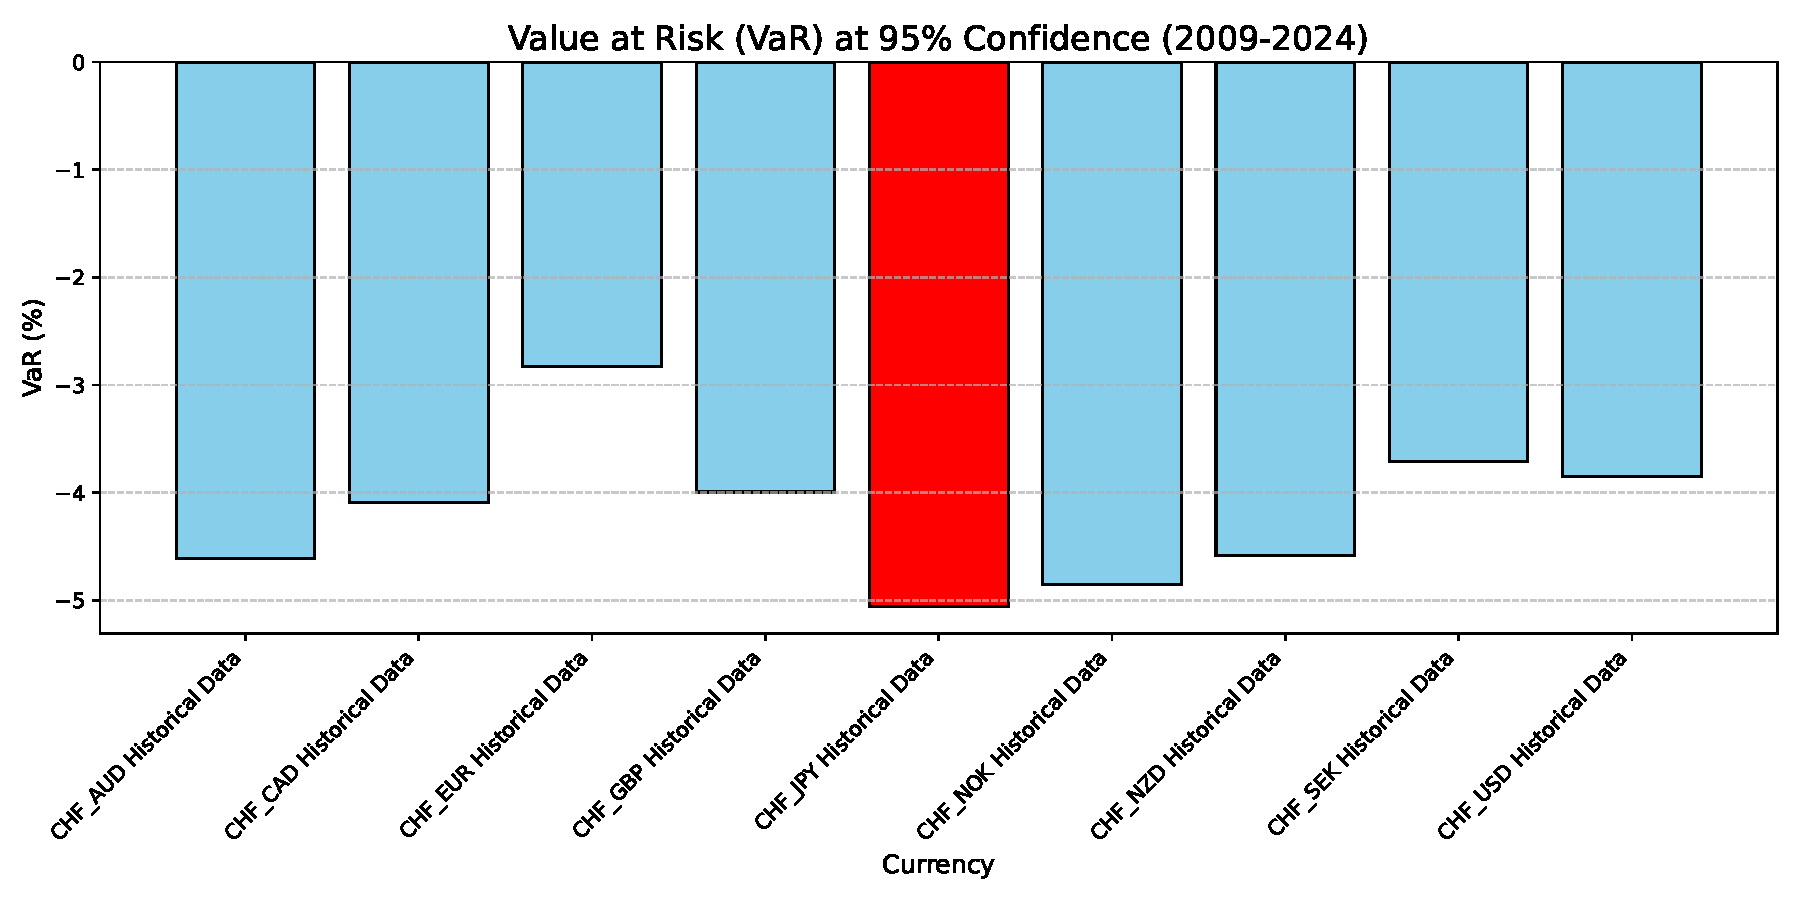
\includegraphics[width=0.75\textwidth]{../../images/var_2009_2024.pdf}
    \caption{Value at Risk of Exchange rates (2009--2024).}
    \label{fig:var_2009_2024}
\end{figure}

The Value at Risk results during this timeframe also underscore the Japanese Yen as the riskiest currency, with a VaR of -5.05\% at a 95\% confidence level. Similarly, the Norwegian Krone recorded a VaR of -4.85\%. This highlights the NOK's pronounced downside risk due to its exposure to volatile oil prices \parencite{bergholt2016business}. In contrast, the Swiss Franc-Euro pair exhibited the lowest VaR at -2.83\%, confirming its relative stability and the continued alignment of economic policies between Switzerland and the eurozone.

The results from the four risk metrics—depreciation, volatility, maximum drawdown, and VaR—highlight the continued sensitivity of smaller and commodity-based currencies like the NOK and NZD to external shocks. Similarly, the Japanese Yen's significant metrics reflect its unique position as a globally traded currency influenced by market sentiment and central bank policies. The Euro and Swiss Franc, on the other hand, demonstrated lower risk across all metrics, reflecting their positions within stable and integrated economic regions. These findings underscore the role of macroeconomic fundamentals and policy stability in shaping currency risks for Swiss investors. Understanding these dynamics is crucial for formulating strategies to mitigate exchange rate risk in diversified portfolios.

\section{Comprehensive Analysis of the Entire Period (2000–2024)}
The comprehensive analysis of the entire period from 2000 to 2024 offers a complete view of the risks associated with the G10 currencies for a Swiss resident. By considering all four metrics, the study identifies the New Zealand Dollar as the riskiest currency during this timeframe. This consistent finding across the metrics highlights the unique challenges posed by this currency for risk management.

\begin{figure}[h!]
    \centering
    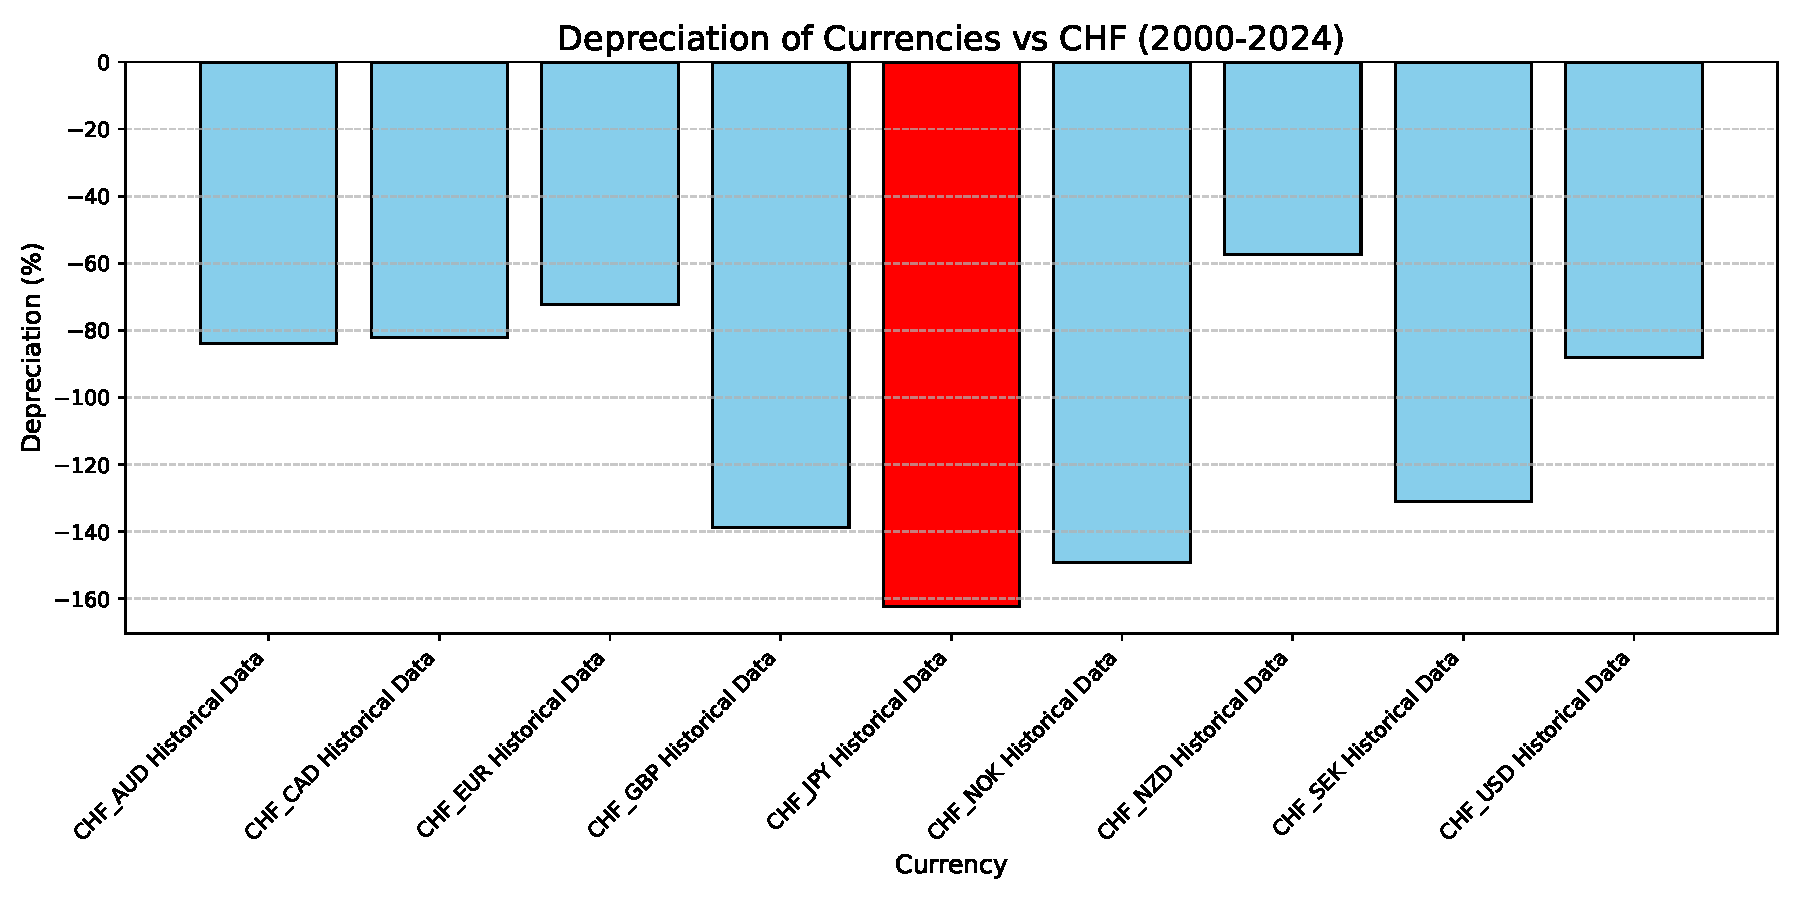
\includegraphics[width=0.75\textwidth]{../../images/depreciation_2000_2024.pdf}
    \caption{Depreciation of Currencies vs CHF (2000--2024).}
    \label{fig:depreciation_2000_2024}
\end{figure}

Starting with depreciation, the Japanese Yen exhibited the most significant depreciation (-162.21\%) relative to the Swiss Franc over the 24-year period. This persistent weakness reflects the Bank of Japan's prolonged monetary easing policies and negative interest rates, which aimed to stimulate domestic growth but devalued the currency in international markets \parencite{shirai2020bank}. In contrast, the New Zealand Dollar demonstrated a relatively lower depreciation (-57.24\%), underlining its better performance against the Swiss Franc despite its exposure to commodity price volatility. The Euro, with a depreciation of -72.38\%, showed relative stability during this period, likely aided by the eurozone's monetary policies and strong economic integration with Switzerland.

\begin{figure}[h!]
    \centering
    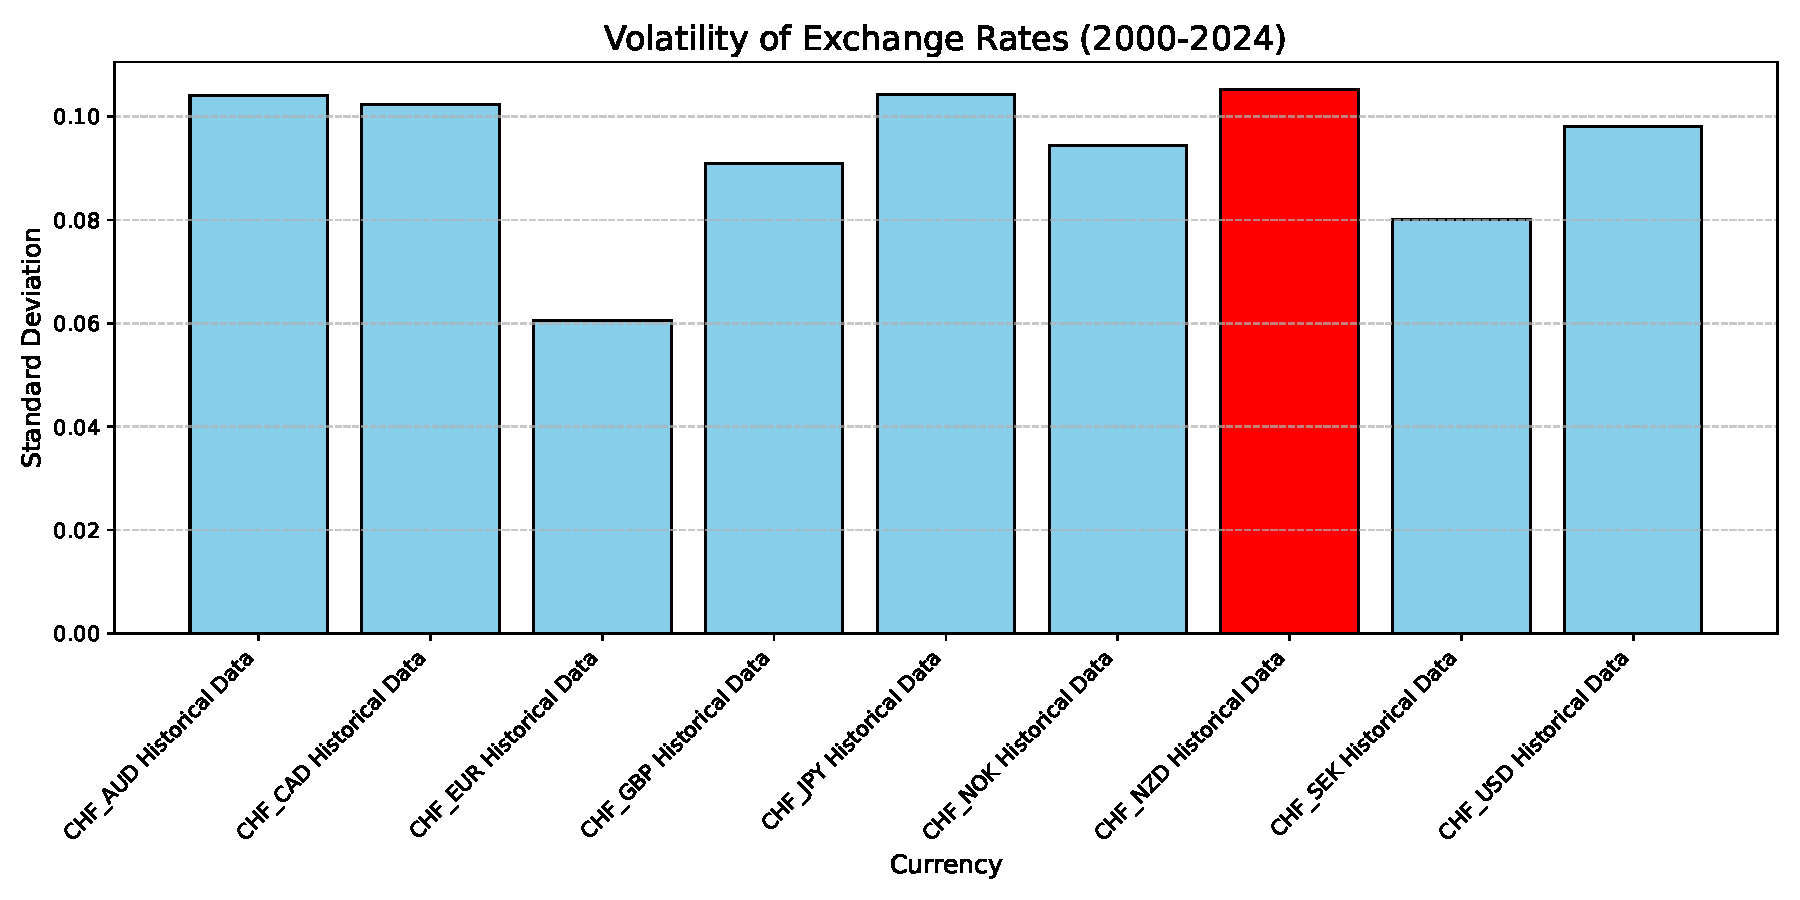
\includegraphics[width=0.75\textwidth]{../../images/volatility_2000_2024.pdf}
    \caption{Volatility of Exchange rates (2000--2024).}
    \label{fig:volatility_2000_2024}
\end{figure}

Turning to volatility, the New Zealand Dollar displayed the highest standard deviation (0.105294), indicating significant fluctuations in its exchange rate over the period. Such high volatility reflects the inherent instability of the New Zealand Dollar, influenced by factors such as commodity price dependencies and a relatively smaller, open economy \parencite{chen2003commodity}. In contrast, the Euro exhibited the lowest volatility (0.060467), underscoring the stability of the Euro in relation to the Swiss Franc. Additionally, the relatively low volatility of the Euro and the Swiss Franc during a portion of the study period can also be attributed to the Swiss National Bank’s (SNB) monetary policy. The Swiss National Bank implemented the minimum exchange rate of CHF 1.20 per Euro from 2011 to 2015, effectively reducing volatility between the Swiss franc and the Euro. This policy contributed to observed stability in exchange rate fluctuations during this time, particularly in the face of broader eurozone uncertainties \parencite{auer2015safe}.

\begin{figure}[h!]
    \centering
    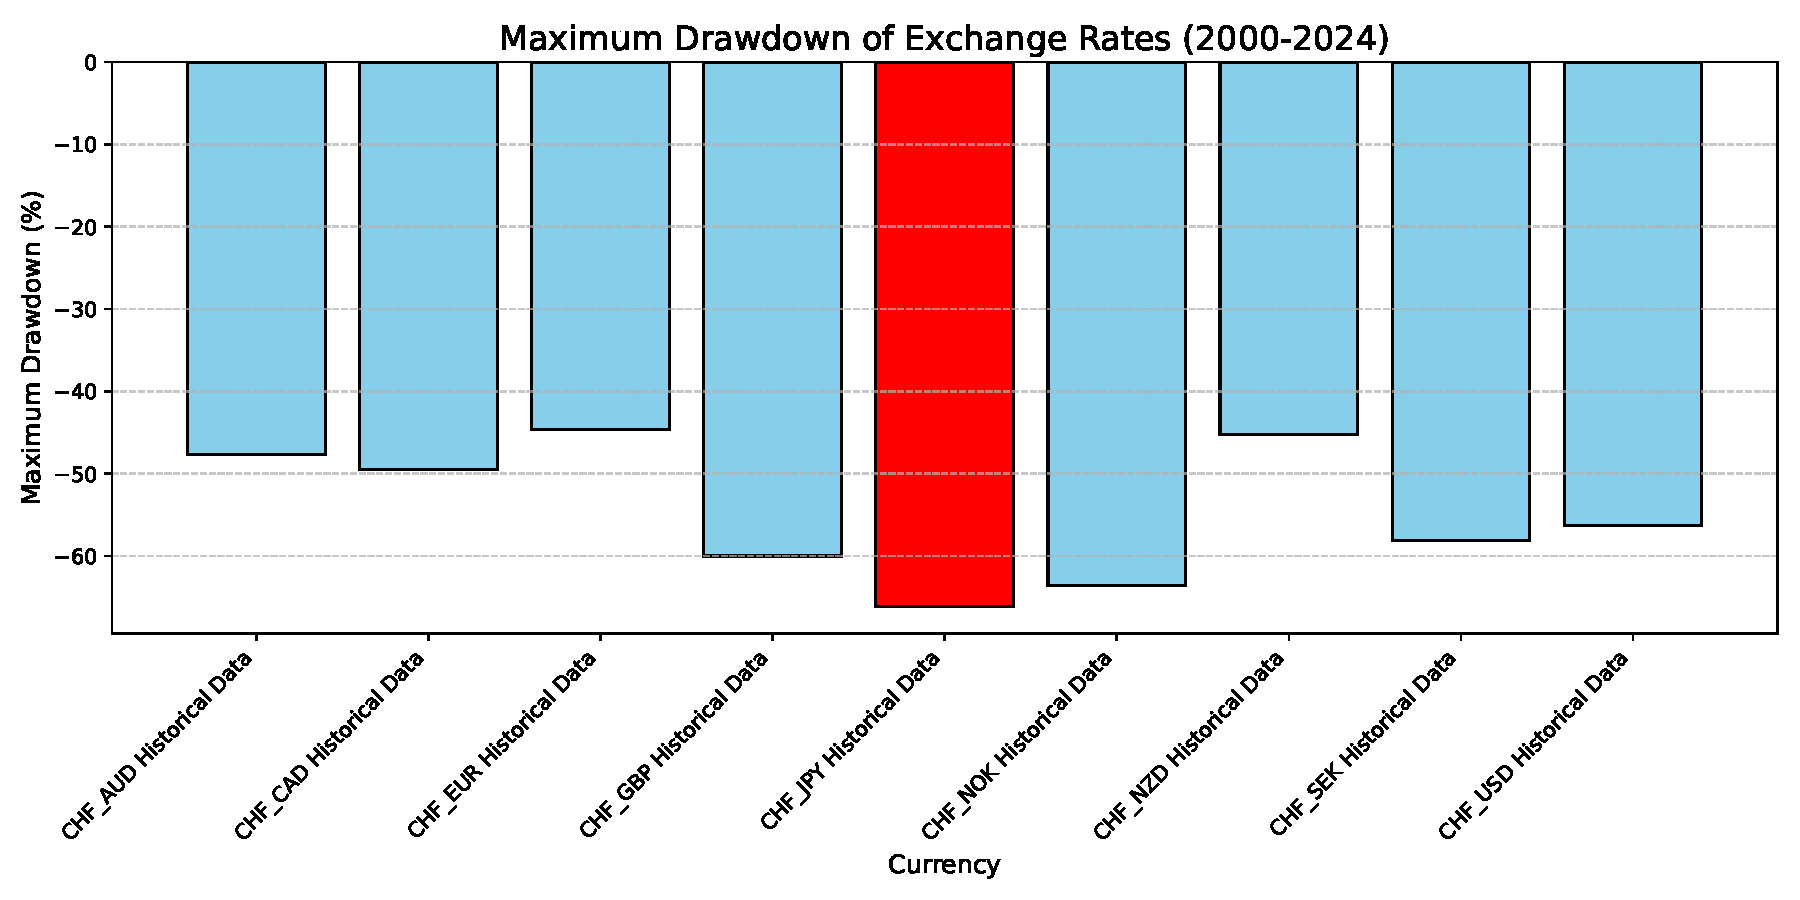
\includegraphics[width=0.75\textwidth]{../../images/maximum_drawdown_2000_2024.pdf}
    \caption{Maximum Drawdown of Exchange rates (2000--2024).}
    \label{fig:maximum_drawdown_2000_2024}
\end{figure}

The maximum drawdown metric further underscores the risks of holding the New Zealand Dollar. With a maximum drawdown of -45.22\%, it demonstrates significant exposure to steep declines in value, reflecting periods of severe economic downturns or external shocks. Similarly, the Norwegian Krone (NOK) displayed a maximum drawdown of -63.62\%, highlighting its sensitivity to oil price fluctuations and dependency on petroleum exports \parencite{bergholt2016business}. The Japanese Yen, contrary to its safe-haven reputation, recorded the steepest maximum drawdown at -66.09\%, likely due to speculative trading and the BOJ's monetary policies weakening the currency's value during critical periods \parencite{shirai2020bank}. By contrast, the Euro experienced the smallest maximum drawdown (-44.60\%), supported by its integration into the stable eurozone economy and relatively conservative monetary policies.

\begin{figure}[h!]
    \centering
    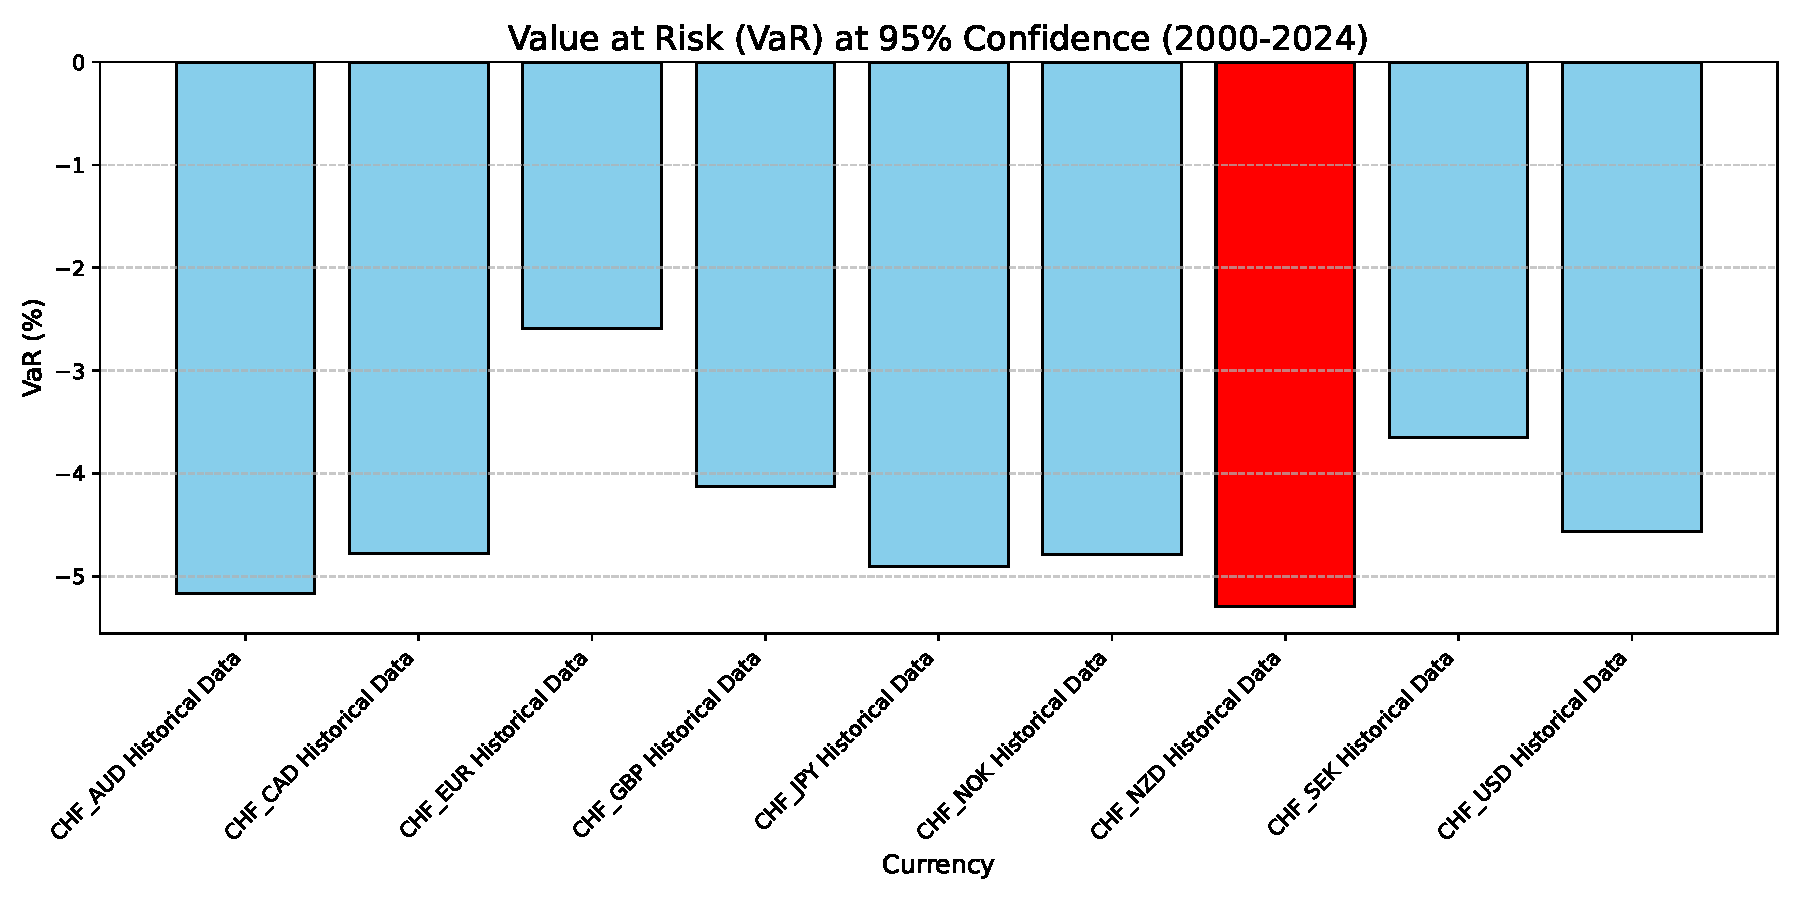
\includegraphics[width=0.75\textwidth]{../../images/var_2000_2024.pdf}
    \caption{Value at Risk of Exchange rates (2000--2024).}
    \label{fig:var_2000_2024}
\end{figure}

Value at Risk (VaR) analysis complements these findings. The New Zealand Dollar emerged as the riskiest currency in terms of VaR, with a maximum expected loss of -5.29\% at a 95\% confidence level. Similarly, the Norwegian Krone demonstrated a VaR of -4.79\%, reflecting its vulnerability to fluctuations in crude oil prices \parencite{bergholt2016business}. The Euro, with a VaR of -2.59\%, maintained its position as the least risky currency, emphasizing its comparative stability over time.

Synthesizing all four metrics provides a nuanced understanding of currency risks over the long term. The Japanese yen's maximum drawdown and fast decline underscore the compromises of its safe-haven status, which frequently results in speculative volatility. Because of its reliance on erratic international markets and susceptibility to external shocks, the New Zealand dollar has continuously been placed among the riskiest currencies across all measures. Strong economic frameworks and well-timed monetary interventions, on the other hand, helped the Euro and Swiss Franc emerge as comparatively stable choices.

These findings are an essential reminder of the variety of variables affecting currency risks and the significance of placing risk evaluations in the context of larger economic frameworks. To reduce exposure to currency risks and make wise financial decisions, Swiss investors must comprehend how depreciation, volatility, maximum drawdown, and VaR interact.

\chapter{Conclusion}
This study aimed to identify the riskiest G10 currency for a Swiss resident by employing four distinct risk metrics: depreciation, volatility, maximum drawdown, and value at risk. Across the four metrics and different timeframes, the analysis consistently identified the Japanese Yen as the riskiest currency. Its pronounced fluctuations and steep depreciation (-162.21\%) underscore the vulnerability to global economic shocks, oil price dependencies, and monetary policy influences. Similarly, the Norwegian Krone (-149.24\% depreciation) was also identified as a high-risk currency, underscoring their vulnerabilities to global economic shocks and oil price dependencies. In contrast, the Euro consistently exhibited the lowest risk levels, attributed in part to the stability of the eurozone economy and the interventionist policies of the Swiss National Bank to maintain exchange rate stability in prior years \parencite{auer2015safe}.

The importance of the selected metrics varies greatly based on the viewpoint of risk evaluation. Depreciation allows for an evaluation of long-term currency strength, particularly useful for investors seeking stability over extended periods. Volatility reflects the degree of variation in exchange rates over time and is especially valuable for recognizing currencies susceptible to instability. Maximum drawdown is ideal for assessing the magnitude of possible losses in severe market declines, providing valuable information on the most unfavorable historical situations. Ultimately, VaR measures potential losses in standard market scenarios at a defined confidence level, rendering it a crucial instrument for organizations handling currency risk within clearly established limits \parencite{hull2012risk}. Collectively, these metrics offer an extensive perspective on currency risks, tackling both ordinary and exceptional market situations.

In addition to the risk metrics, broadening the dataset before 2000 or adding other elements like geopolitical risks, differences in monetary policy, or macroeconomic indicators might offer a more detailed analysis. For instance, event studies examining particular crises, like the 2008 financial collapse or the 2020 COVID-19 pandemic, may uncover how these shocks distinctly impact currency risks as time progresses. Furthermore, the role of interventionist policies, such as those by the Swiss National Bank during the eurozone debt crisis, could be examined to provide a deeper understanding of their long-term effects on currency risks. Additionally, utilizing machine learning models to predict exchange rate risks by analyzing historical trends and economic signals could open up new paths for improving forecasting precision.

In summary, this study underscores the comparative risks of G10 currencies for Swiss investors, emphasizing the necessity of customizing risk evaluations to align with individual investor requirements and economic contexts. The results highlight the diverse aspects of currency risk and the necessity for a comprehensive range of metrics and methods to address its complexity. As financial markets evolve, it will be crucial to incorporate more data sources and sophisticated analytics to enhance our comprehension of currency risks and support informed decision-making.

\printbibliography

\end{document}
